\clearpage
\section{Sample selection}
\label{sec:Sample_selection}

\subsection{MUSE-GTO MAGIC}

\subsection{COSMOS field}

\begin{table}[htbp]

	\hspace{50pt}

	\begin{tabular}{ccccccc}
	\hline
	Group & Ra\textsuperscript{2} & Dec\textsuperscript{3} & Exposure\textsuperscript{4}  & Average & Total nb. & Nb. field \\
	
	ID\textsuperscript{1} & J2000 (\degree) & J2000 (\degree) & (hr) & seeing\textsuperscript{5} (") & galaxies\textsuperscript{6} & galaxies\textsuperscript{7} \\	
	
	\hline
	\hline
	CGr32 & NaN & NaN & $3 \times 4.35$ & $0.51$ - $0.58$ & NaN & NaN \\
	\hline
	CGr34\_d & $149.87766$ & $2.502331$ & $5.25$ & $0.63$ & NaN & NaN \\
	\hline
	CGr34\_bs & $149.87766$ & $2.502331$ & $4.75$ & NaN & NaN & NaN \\
	\hline
	CGr30\_d & $150.144225$ & $2.065971$ & $9.75$ & $0.67$ & NaN & NaN \\
	\hline
	CGr30\_bs & $150.144225$ & $2.065971$ & $6.25$ & NaN & NaN & NaN \\
	\hline
	CGr84 & $150.057219$ & $2.599744$ & $5.25$ & $0.59$ & NaN & NaN \\
	\hline
	CGr84-N & NaN & NaN & $1$ & $0.51$ & NaN & NaN \\
	\hline
	CGr114 & $149.994285$ & $2.258044$ & $2.2$ & $0.68$ & NaN & NaN \\
	\hline
	CGr79 & $149.820686$ & $1.821825$ & $4.35$ & $0.60$ & NaN & NaN \\
	\hline
	CGr28 & $150.218094$ & $1.812667$ & $1$ & $0.62$ & NaN & NaN \\
	\hline
	CGr26 & $150.492767$ & $2.069139$ & $1$ & $0.59$ & NaN & NaN \\
	\hline
	CGr61 & $149.728741$ & $1.915987$ & $1$ & $0.64$ & NaN & NaN \\
	\hline
	CGr51 & $149.982756$ & $1.801899$ & $1$ & $0.6-0.7$ & NaN & NaN \\
	\hline
	CGr23 & $149.790782$ & $2.162648$ & $1$ & $0.68$ & NaN & NaN \\
	\hline
	
	\end{tabular}
	
	\caption[Main characteristics of the observed MUSE fields]{\label{table:MUSEfieldsProp}Main characteristics of the observed MUSE fields. Groups ending with \_d correspond to deep observations (full stacked OBs) and with \_bs correspond to best-seeing observations (only OBs with a seeing below $\SI{0.7}{"}$). The seeing is given for the [OII] wavelength at the group's redshift. 1. MUSE group number, 2. Group centre's right ascension, 3. Group centre's declination, 4. Duration of observations, 5. Average seeing during observation, 6. Total number of detected galaxies within MUSE FoV, 7. Number of field galaxies found by the FoF algorithm.}
\end{table}

The point of the analysis is to perform a joint study of the morphology and the kinematics of field galaxies in COSMOS \shortcite{Scoville2007} using respectively HST ACS images and MUSE data. To this end, a set of $12$ galaxy structures (these can be either groups or clusters) in COSMOS was selected. The choice of the COSMOS field for this analysis was made because of the large number of multi-band photometric data available for the galaxies in this field and the presence of rich (large number of member galaxies) galaxy groups.\\

Guaranteed Time Observations (GTO) centred on the groups were performed from which 14 different MUSE Fields of View (FoV) of $1 \times \SI{1}{arcmin^2} $ were obtained. Each is composed of Observation Blocks (OB) of \textcolor{red}{$\SI{30}{min}$} each with the Position Angle (PA) of the instrument rotated by $\SI{90}{\degree}$ between consecutive observations.

Most of the groups are in one FoV, except for CGr32. Since this group is \textcolor{red}{larger} than the others, three slightly overlapping FoVs were taken around it. A couple of groups were also split into \textit{deep} and \textit{best-seeing} observations, the former combining all the OBs regardless of the average seeing in each OB, when the latter only kept OBs with an average seeing higher than $\SI{0.7}{"}$.

 The main characteristics of the observed FoVs, including the position of their centre, the exposure per FoV, the average seeing during the observation, the total number of galaxies and the number of field galaxies detected by the FoF algorithm are listed in Table\,\ref{table:MUSEfieldsProp}. \\

These structures were chosen within the COSMOS field. This ensured them to have both a large set of corresponding photometric data available from \shortciteA{laigle_cosmos2015_2016} catalogue and HST images with a much better resolution (\SI{0.03}{arcsec/px} for HST and $\sim \SI{0.2}{arcsec/px}$ for MUSE). A few galaxies in CGr30\_deep and around some stars might have also been detected within the data cubes but not in HST images. In the former case, the reason is that a blind source detection was performed with ORIGIN \shortcite{Bacon2017} which can deblend sources even below the PSF. For the latter, this is because galaxies were detected in areas around stars which were masked when creating \shortciteA{laigle_cosmos2015_2016} catalogue.

\subsection{Prior information on the galaxies}

\subsubsection{Galaxies in structures}

This internship was planned to be similar in many aspects to what has done V. Abril-Melgajero in LAM, Marseille. She studied the morphology and the kinematics of the galaxies within the structures observed by MUSE in COSMOS. The galaxies were therefore found in the same MUSE fields as those we are using in this work, but belong to structures instead of being labelled as \textcolor{red}{field galaxies}. 

To differentiate between group and field galaxies, a Friend of Friends algorithm (FoF) was run prior to my arrival on the galaxies in each MUSE field. Thus, each galaxy was labelled either as belonging to a structure or as field galaxies.

Additionnaly, a morphological analysis had already been performed by V. Abril-Melgajero with GALFIT on galaxies in structures. Two Sérsic profiles with fixed Sérsic indices ($n = 1, 4$) were used to describe these galaxies as a combination of a disk and a bulge component. Hence, their intensity can be written as

\begin{equation}
	I(r) = I_{e, \rm{d}} \, e^{-b_1 \left [ \frac{r}{R_{\rm{d}}} -1 \right ]} + I_{e , \rm{b}} e^{- b_4 \left [ \left ( \frac{r}{R_{\rm{b}}} \right )^{1/4} -1 \right ]}
	\label{eq:GALFIT_light_profile}
\end{equation}
where $I_{e, \rm{d}}$, $I_{e, \rm{b}}$ are the effective intensities of the disk and the bulge component respectively and $R_{\rm{d}}$, $R_{\rm{b}}$ their half-light radii.

Therefore, we already had morphological information for roughly half of the total sample including model parameters as described above, but also morphological parameters such as the ellipticity of the galaxies, the Position Angle (PA) of their kinematical main axis (which can be different from the morphological PA).

\subsubsection{Morphological information from COSMOS catalogues}

The total number of galaxies detected by MUSE in COSMOS is around $1000$. Roughly half of them belong to structures and the other half are labelled as field galaxies. Among these galaxies, not all of them are useful to our study. Some may be too close to the edge, others be too noisy with a low Signal to Noise Ratio (SNR), or too small for any relevant kinematical modelling. It is thus mandatory to apply a selection on our data set of field galaxies, first to save time for the analysis, but also to reduce uncertainties.

Our goal is to perform a joint study of the morphology and the kinematics of these galaxies. The tools and the models for the kinematical modelling were already developed as they were used by V. Abril-Melgajero. On the other hand, fitting morphological models with software such as GalFit or SExtractor would have required additional time which we did not have. Hopefully for us, morphological modelling had already been performed on the galaxies in the COSMOS field, so we could focus on the kinematical part. \\

Morphological information for all the galaxies in COSMOS can be found in various catalogues and tables\footnote{\url{https://irsa.ipac.caltech.edu/data/COSMOS/tables/morphology/}}. To start with, we decided to use the two most complete catalogues we could find, that of Tasca (maybe citation) and Cassata (maybe citation as well). Both catalogues contain morphological information including the central position of the galaxy, its half-light radius, concentration and asymmetry parameters, ellipticity, Position Angle of the major morphological axis (PA), and many more for roughly $232 000$ galaxies. The authors obtained morphological information by running SExtractor on HST images of the galaxies in \shortciteA{laigle_cosmos2015_2016} catalogue. \\

Since we already had data from \shortciteA{laigle_cosmos2015_2016} for our galaxies, we only had to cross-match our table with Cassata's and Tasca's catalogues to collect their morphological parameters. We decided to cross-match our data with each catalogue separately and then with both using the right ascension $\alpha$ and declination $\delta$ of the centre of the galaxies, allowing for a maximum separation between the MUSE source and the closest source within Cassata's and Tasca's catalogues of $\SI{1}{arcsec}$ maximum. 

This cross-matching procedure was performed for both field and structure galaxies. The reason for cross-matching cluster galaxies when we are only interested in those in the field will be discussed in the following section.

\subsection{Checking catalogues values consistency}
\subsubsection{Reasons for checking catalogues values}

\begin{figure}[H]
	\centering
	\begin{minipage}[c]{0.49\linewidth}
		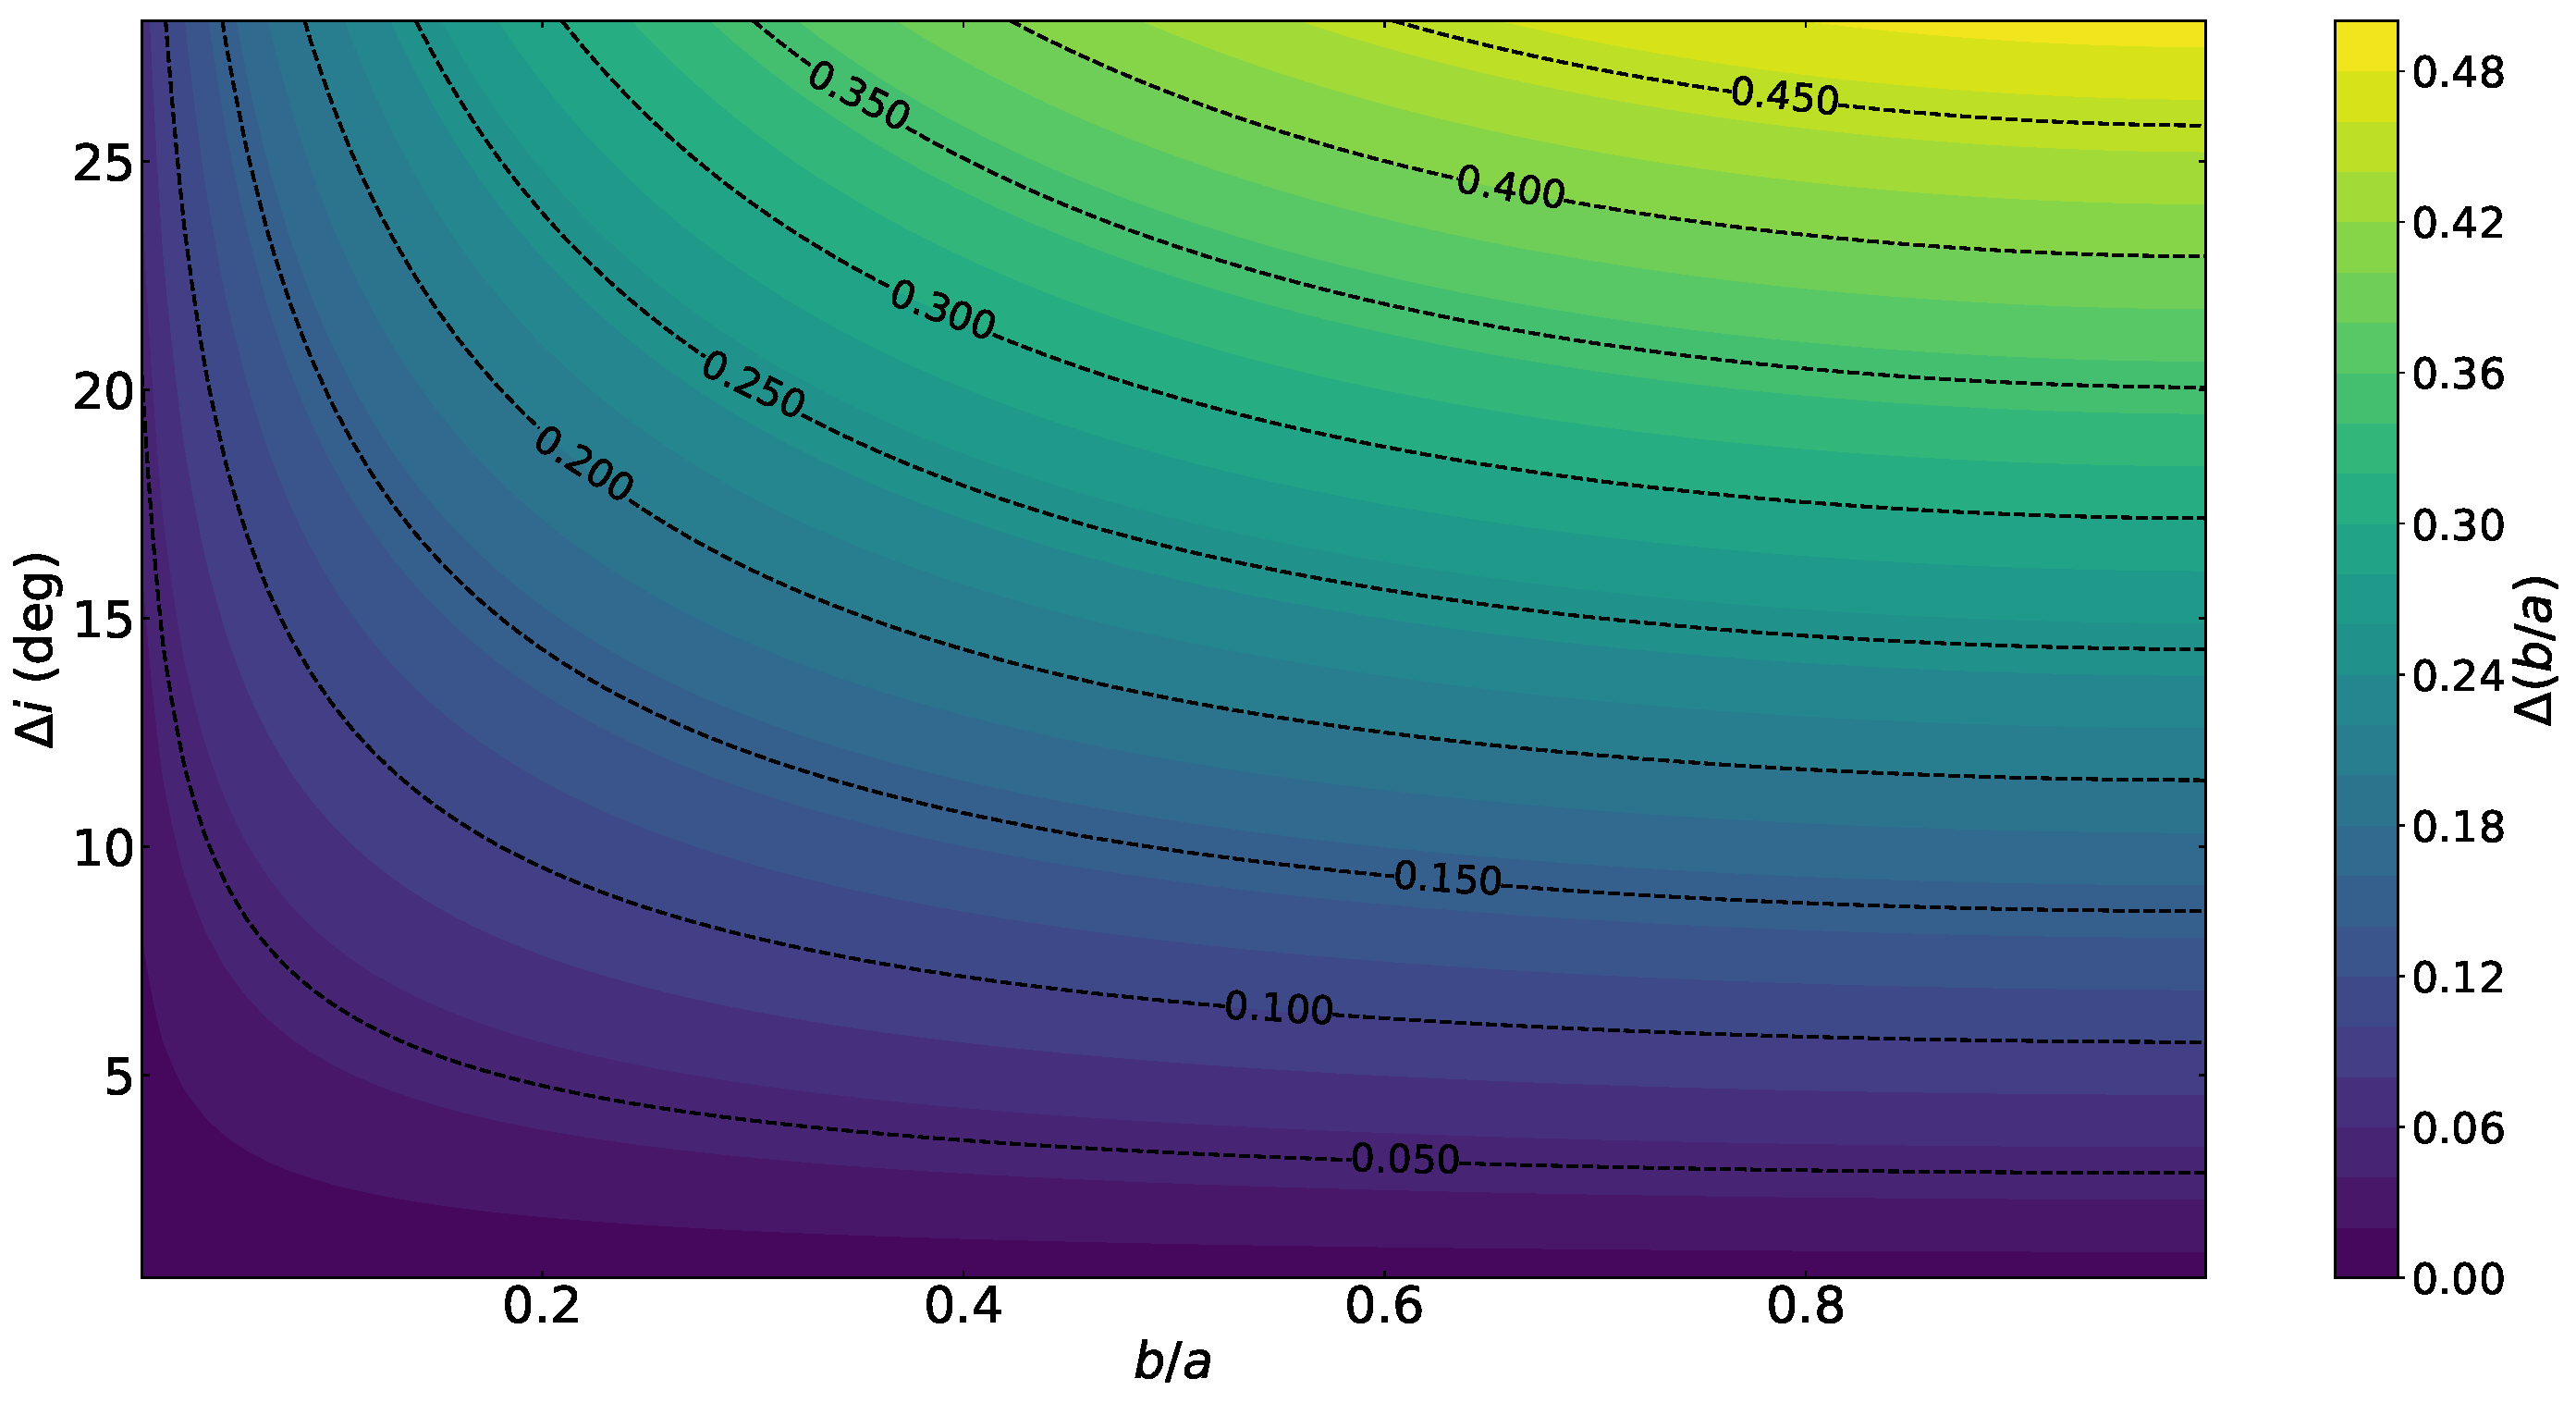
\includegraphics[width=\linewidth]{../Plots/Error_on_inc_versus_b_a.pdf}
		\subcaption{Error on inclination as a function of $b/a$ and its absolute error. Contours of $\Delta (b/a)$ are plotted in black dashed lines with their corresponding value.}
	\end{minipage}
	\hfill
	\begin{minipage}[c]{0.49\linewidth}
		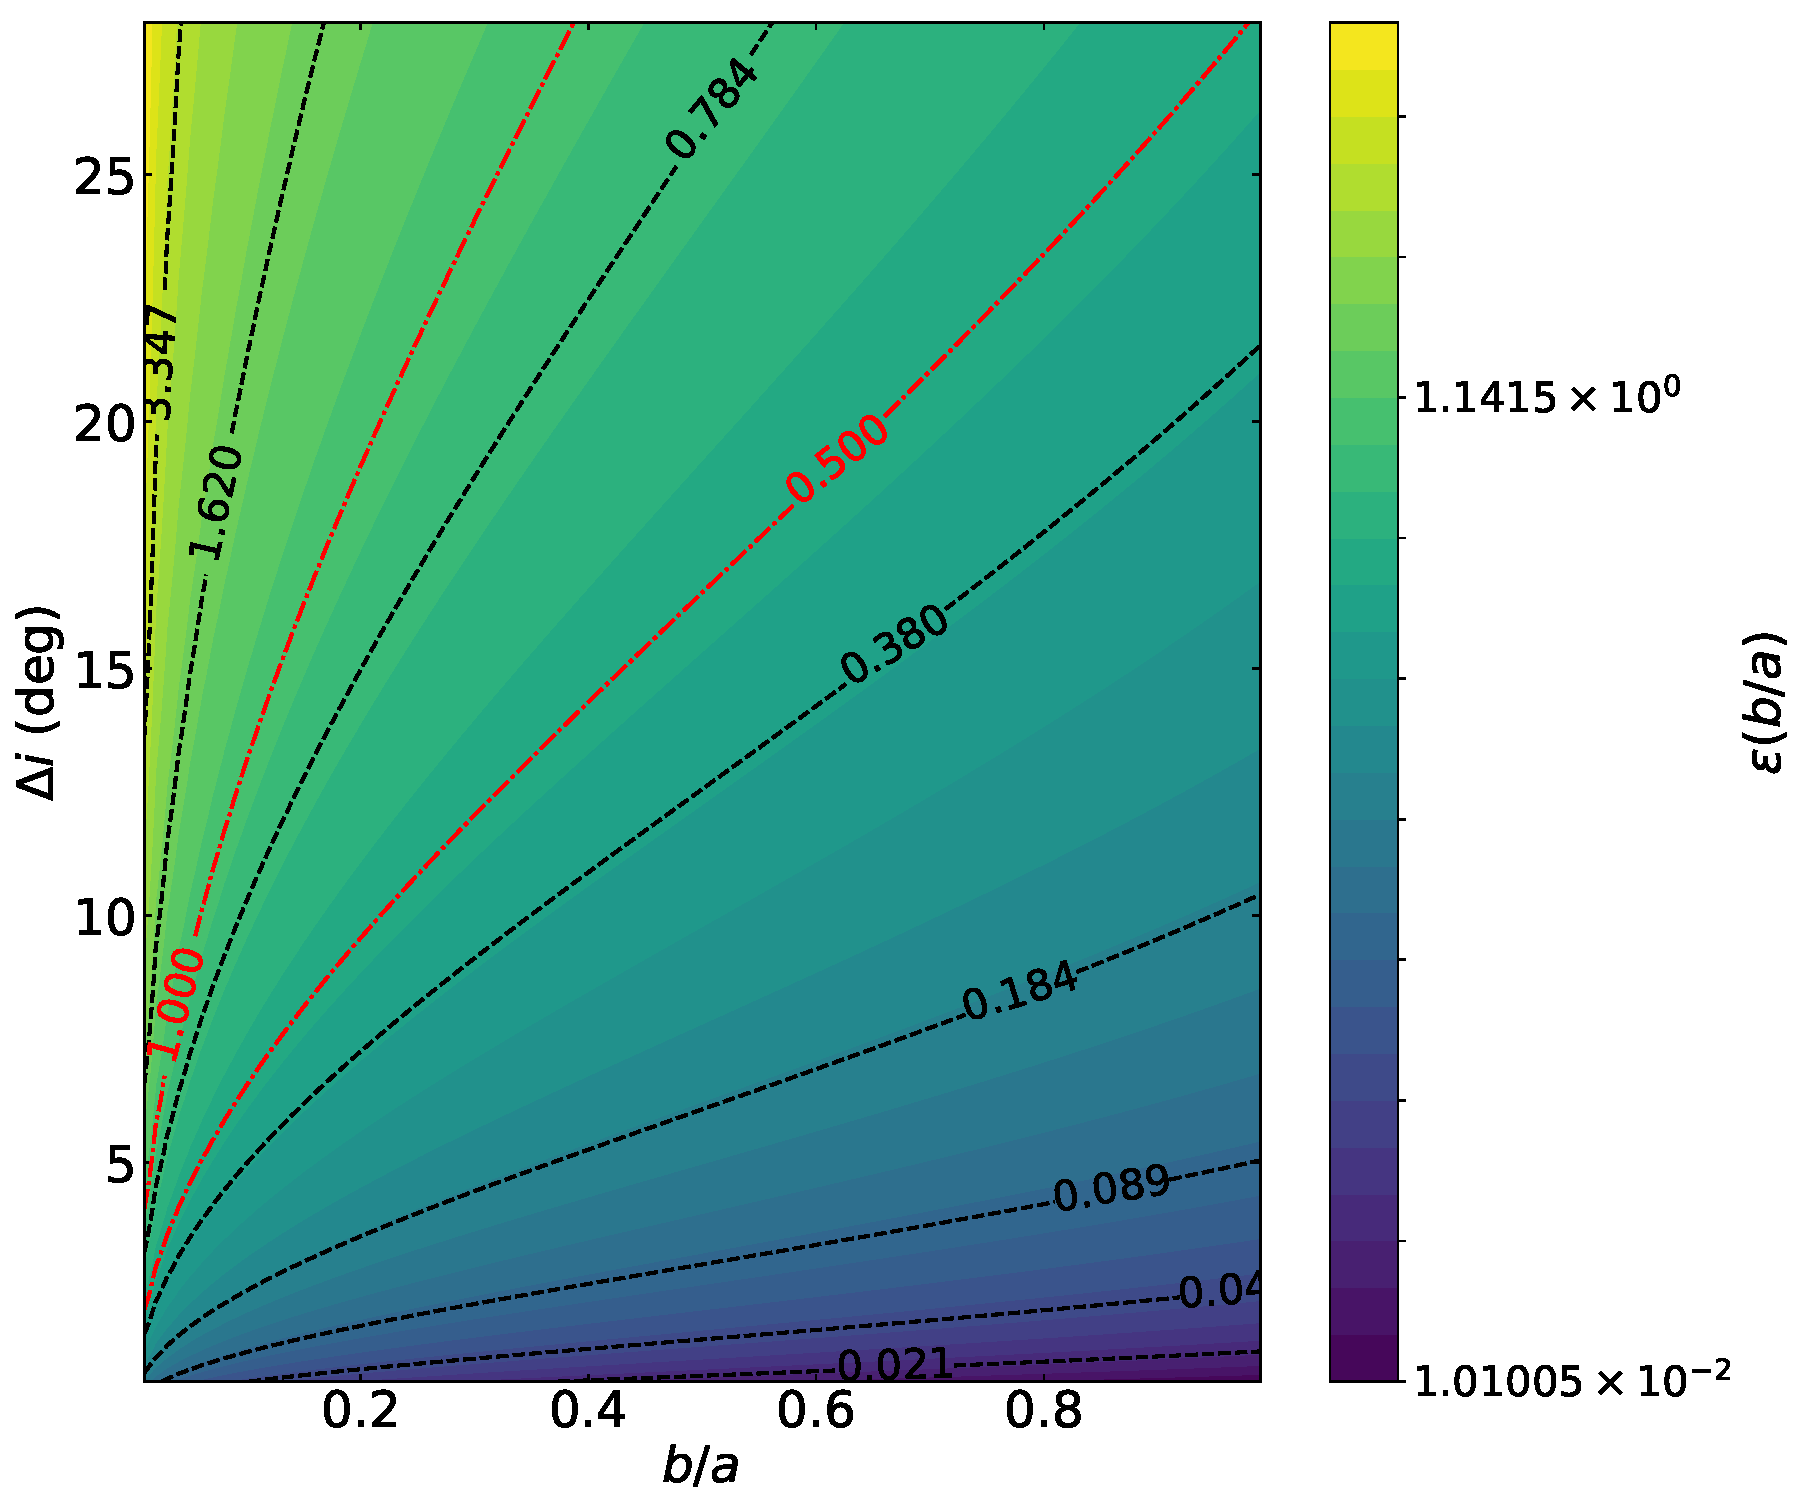
\includegraphics[width=\linewidth]{../Plots/RelError_on_inc_versus_b_a.pdf}
		\subcaption{Error on inclination as a function of $b/a$ and its relative error. Contours of $\epsilon (b/a)$ are plotted in black and red dashed lines with their corresponding value.}
	\end{minipage}
	\caption[Error on inclination as a function of $b/a$ and its error.]{Error on inclination as a function of $b/a$ and its error. Left: as a function of the absolute error on $b/a$ ($\Delta (b/a)$). Right: as a function of the relative error on $b/a$ ($\epsilon ( b/a)$). Red contours correspond to values for which there is a 50\% and 100\% error on $b/a$.}
	\label{fig:erreur_inclinaison}
\end{figure}

As a first step, we must select a sample based on relevant criteria. This is meant to ensure us to have reliable morphological and kinematical parameters and to reduce statistical errors. Given that any kinematical modelling relies on prior morphological information (galaxy centre, ellipticity, $\rm{PA}$), we can only use a combination of values derived from spectral fitting, for instance the Signal to Noise Ratio ($\rm{SNR}$) as described in Eq.\,\ref{eq:SNR}, and morphological modelling such as a measure of a galaxy radius to select our sample.  

Before this internship, spectral fitting on the integrated spectra of the galaxies had already been done, and we combined our data with morphological information from COSMOS catalogues as discussed in the previous section. Potentially useful morphological information included half-light radii, magnitudes, ratios of minor to major axis ($b/a$) or equivalently a measure of the ellipticity of the galaxies. Nevertheless, using this data without checking first how well it compares to values found in other catalogues and/or derived using different softwares/models could lead to high biases and uncontrolled errors. Thus, before discussing any selection criteria for our sample, we must first assess the reliability of the parameters we are going to use in later sections. \\

Important values to check are the half-light radius, as it will be used to select our sample, the $b/a$ ratio and the $\rm{PA}$ since these are prior information for the kinematical modelling. We also checked that there was a correlation between GALFIT and the catalogues magnitudes. The axes ratio has a crucial importance since it is directly related to the inclination of the galaxy on the sky through Eq.\,\ref{eq:inclinaison}. Given a certain error $\Delta (b/a)$, and using the usual formula for computing the error $\Delta f = | \partial_x f | \Delta x$ of a function $f$, we find for the inclination

\begin{equation}
	\Delta i = \Delta (b/a) \left | \frac{b}{a} \left ( 2 - \frac{b}{a} \right ) \right | ^{-1/2}
\end{equation}

This is illustrated in Fig.\,\ref{fig:erreur_inclinaison} where $\Delta i$ has been plotted as a function of $b/a$ and its error (absolute on the left, relative on the right). Contours of the error on $b/a$ have been over-plotted to show how evolves $\Delta i$ given a fixed error on $b/a$. As expected, the higher the error on $b/a$ the higher the error on $i$. An error as high as 50\% could yield $\Delta i \approx \SI{27}{\degree}$, though this value is reached for $b/a \approx 1$ where the axes ratio is the least constrained by the morphology. A more appropriate error on $b/a$ of 20\% gives a maximum $\Delta i$ slightly above $\SI{10}{\degree}$, which is correct. 

Since the inclination affects the galaxy maximum rotational velocity, and so potentially on the classification of galaxies as rotationnaly supported or dispersion dominated (see Section insert ref here), this indicates us that for any proper kinematical modelling we must check carefully that the values of axes ratios are consistent between catalogues.

\subsubsection{Catalogues used for comparison}

As stated in previous sections, we cross-matched our catalogue of galaxies detected by MUSE in COSMOS with Cassata's and Tasca's, two tables with morphological information for the galaxies in \shortciteA{laigle_cosmos2015_2016}. 

However, as can be seen in Fig.\,\ref{fig:comp_radii} and \ref{fig:comp_radii_with_bulge_or_disk_radius}, we found large discrepancies between the parameters. Thus, to better understand their origin, we chose to cross-match our catalogue with another one (also based on \shortciteA{laigle_cosmos2015_2016}) from Zurich. This table has fewer HST counterparts of MUSE galaxies than in the other two but it contains additional morphological information which we can use for the comparison. 

In addition to that, we already had GALFIT morphological information on $\sim 500$ group galaxies with strong confidence in their value. Therefore, we chose to compare the data in the three morphological catalogues based on \shortciteA{laigle_cosmos2015_2016} with that of GALFIT.

\subsubsection{Total magnitudes}

\begin{figure}[htbp]
	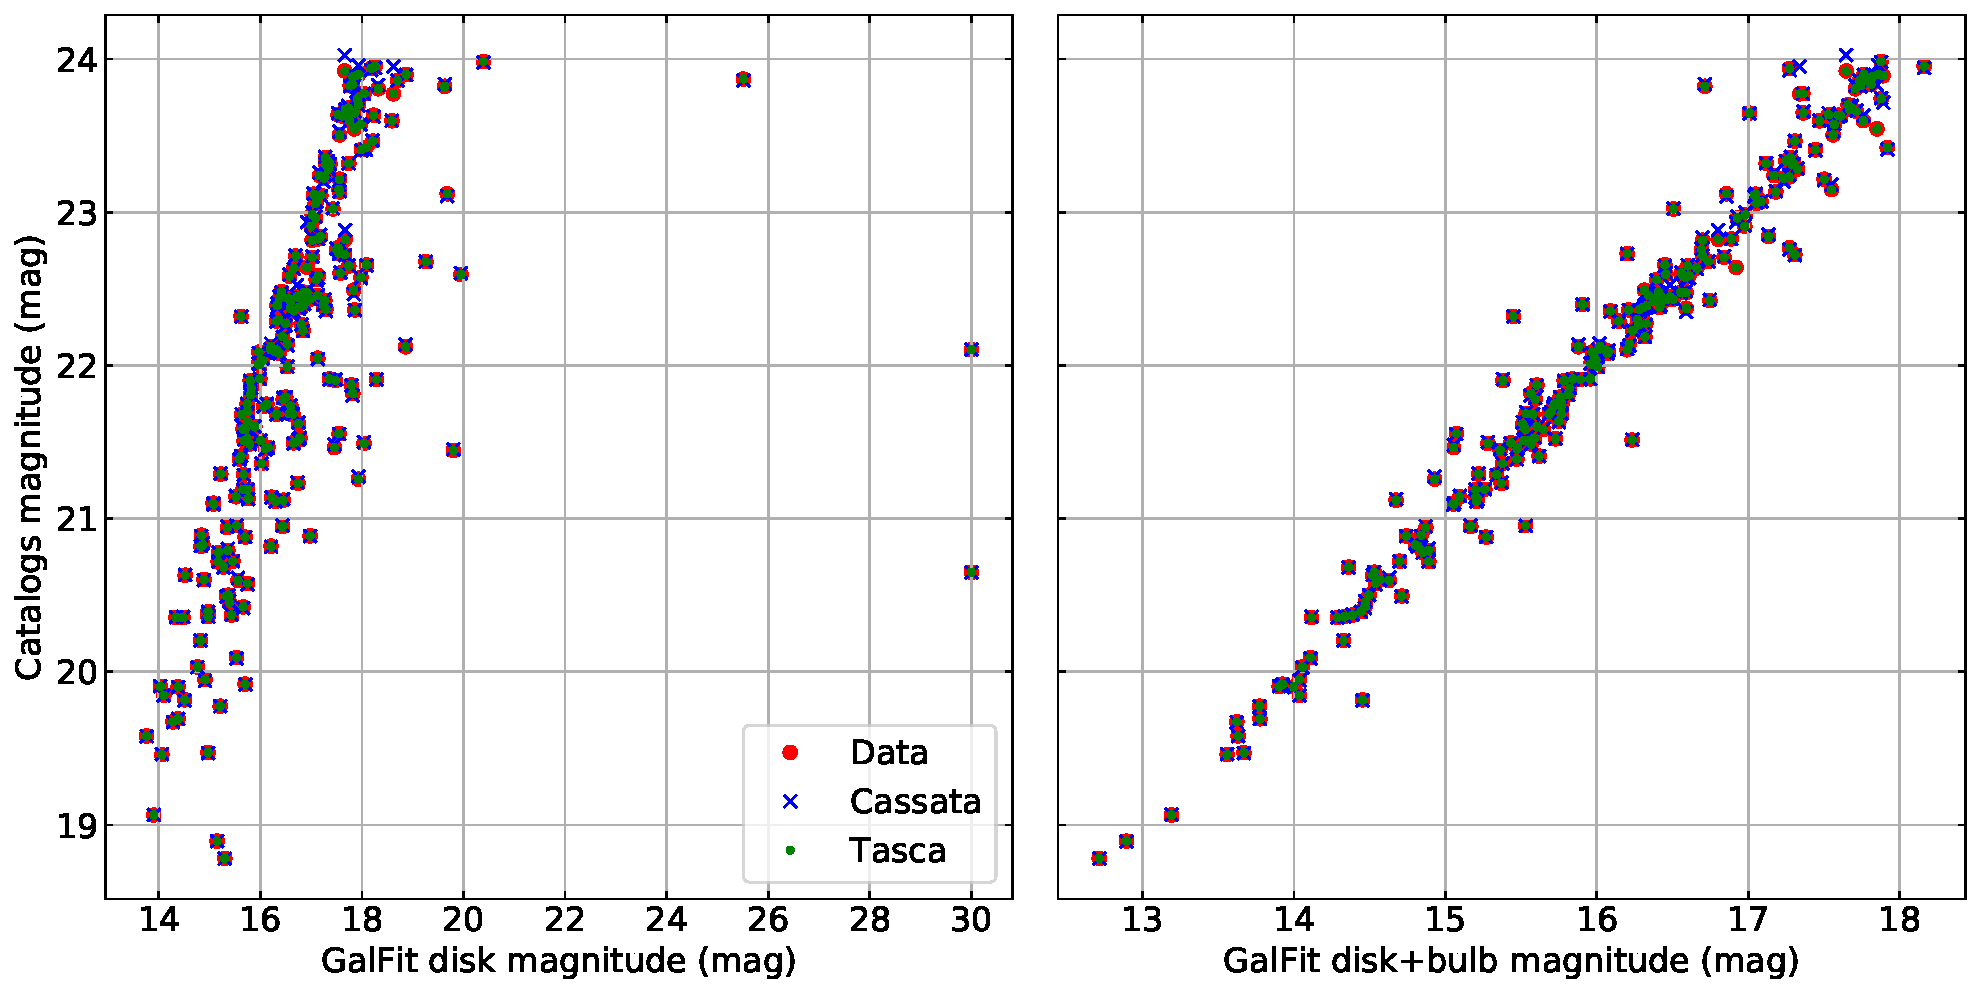
\includegraphics[width=\linewidth]{../Plots/catalogMag_against_GalfitMag_corrected.pdf}
	\caption[Comparison between magnitudes]{Comparison between the morphological catalogues magnitudes and that of GALFIT for cluster galaxies. Magnitudes from the catalogues agree well between each other. Left: compared with GALFIT disk magnitude only. The slope is too high and a few points are scattered far from the line. Right: compared with the total GALFIT magnitude as defined in Eq.\,\ref{eq:tot_mag_final_version}. We find a linear relation with a scatter of about $\SI{1.6}{mag}$.}
	\label{fig:comp_mags}
\end{figure}

The first value we can easily compare is the total magnitude. Cassata's, Tasca's and Zurich's catalogues provide a measure of the total magnitude derived from fitting with SExtractor a single Sérsic profile with a free Sérsic index $n$ on HST images.

Given that GALFIT light profile was modelled using two Sérsic profiles with fixed Sérsic indices ($n = 1, 4$), we had two measures of the magnitude of these galaxies: one for the bulge component $m_{\rm{b}}^{\rm{GF}}$, and another for the disk component $m_{\rm{d}}^{\rm{GF}}$. To have a meaningful comparison between magnitudes, we need to compute the GALFIT total magnitude by combining the bulge and the disk components. Both are defined as

\begin{equation}
	m_i^{GF} = -2.5 \log_{10} \left ( F_i^{\rm{GF}} \right ) + \rm{C}
	\label{eq:disk_bulge_lum}
\end{equation}
 where $i = \rm{b, d}$ represents either the bulge or the disk, $F = L/{4 \pi D^2}$ is the flux of the galaxy in some band, $L$ its intrinsic luminosity, $D$ its cosmological luminosity distance to us and $\rm{C}$ a constant depending on the band used.

Considering that the two components have different luminosities but are located at the same distance, we can add the fluxes together. Thus the total GALFIT magnitude can also be written as

\begin{equation}
	m_{\rm{tot}}^{\rm{GF}} = - 2.5 \log_{10} \left ( F_{\rm{b}}^{\rm{GF}}  + F_{\rm{d}}^{\rm{GF}} \right ) + \rm{C}
	\label{eq:tot_mag}
\end{equation}

Inverting Eq.\,\ref{eq:disk_bulge_lum} to get the components flux as a function of their magnitude and inserting it into Eq.\,\ref{eq:tot_mag} yields

\begin{equation}
	m_{\rm{tot}}^{\rm{GF}} = -2.5 \log_{10} \left [ 10^{-\frac{m_{\rm{b}}}{2.5}} + 10^{-\frac{\rm{m_d}}{2.5}} \right ]
	\label{eq:tot_mag_final_version}
\end{equation}

This is the value that should be compared with the three catalogues magnitudes. Fig.\,\ref{fig:comp_mags} shows how these scale with each other and with GALFIT disk magnitude on the left, and the total magnitude from Eq.\,\ref{eq:tot_mag_final_version} on the right. As expected, the catalogues give the same value except for a few points. We see that the total GALFIT magnitude gives a much better, poorly scattered linear relation with the catalogues magnitudes. Even though there is an offset between GALFIT and the catalogues, this is due to using different conventions for the constant term in Eq.\,\ref{eq:disk_bulge_lum}.

The same comparison was done on field galaxies, except we did not have GALFIT magnitudes in this case. We also found a good agreement between the catalogues magnitudes.

\subsubsection{Morphological type classification}
\label{subsubsec:classification}

\begin{figure}[htbp]
	\centering
	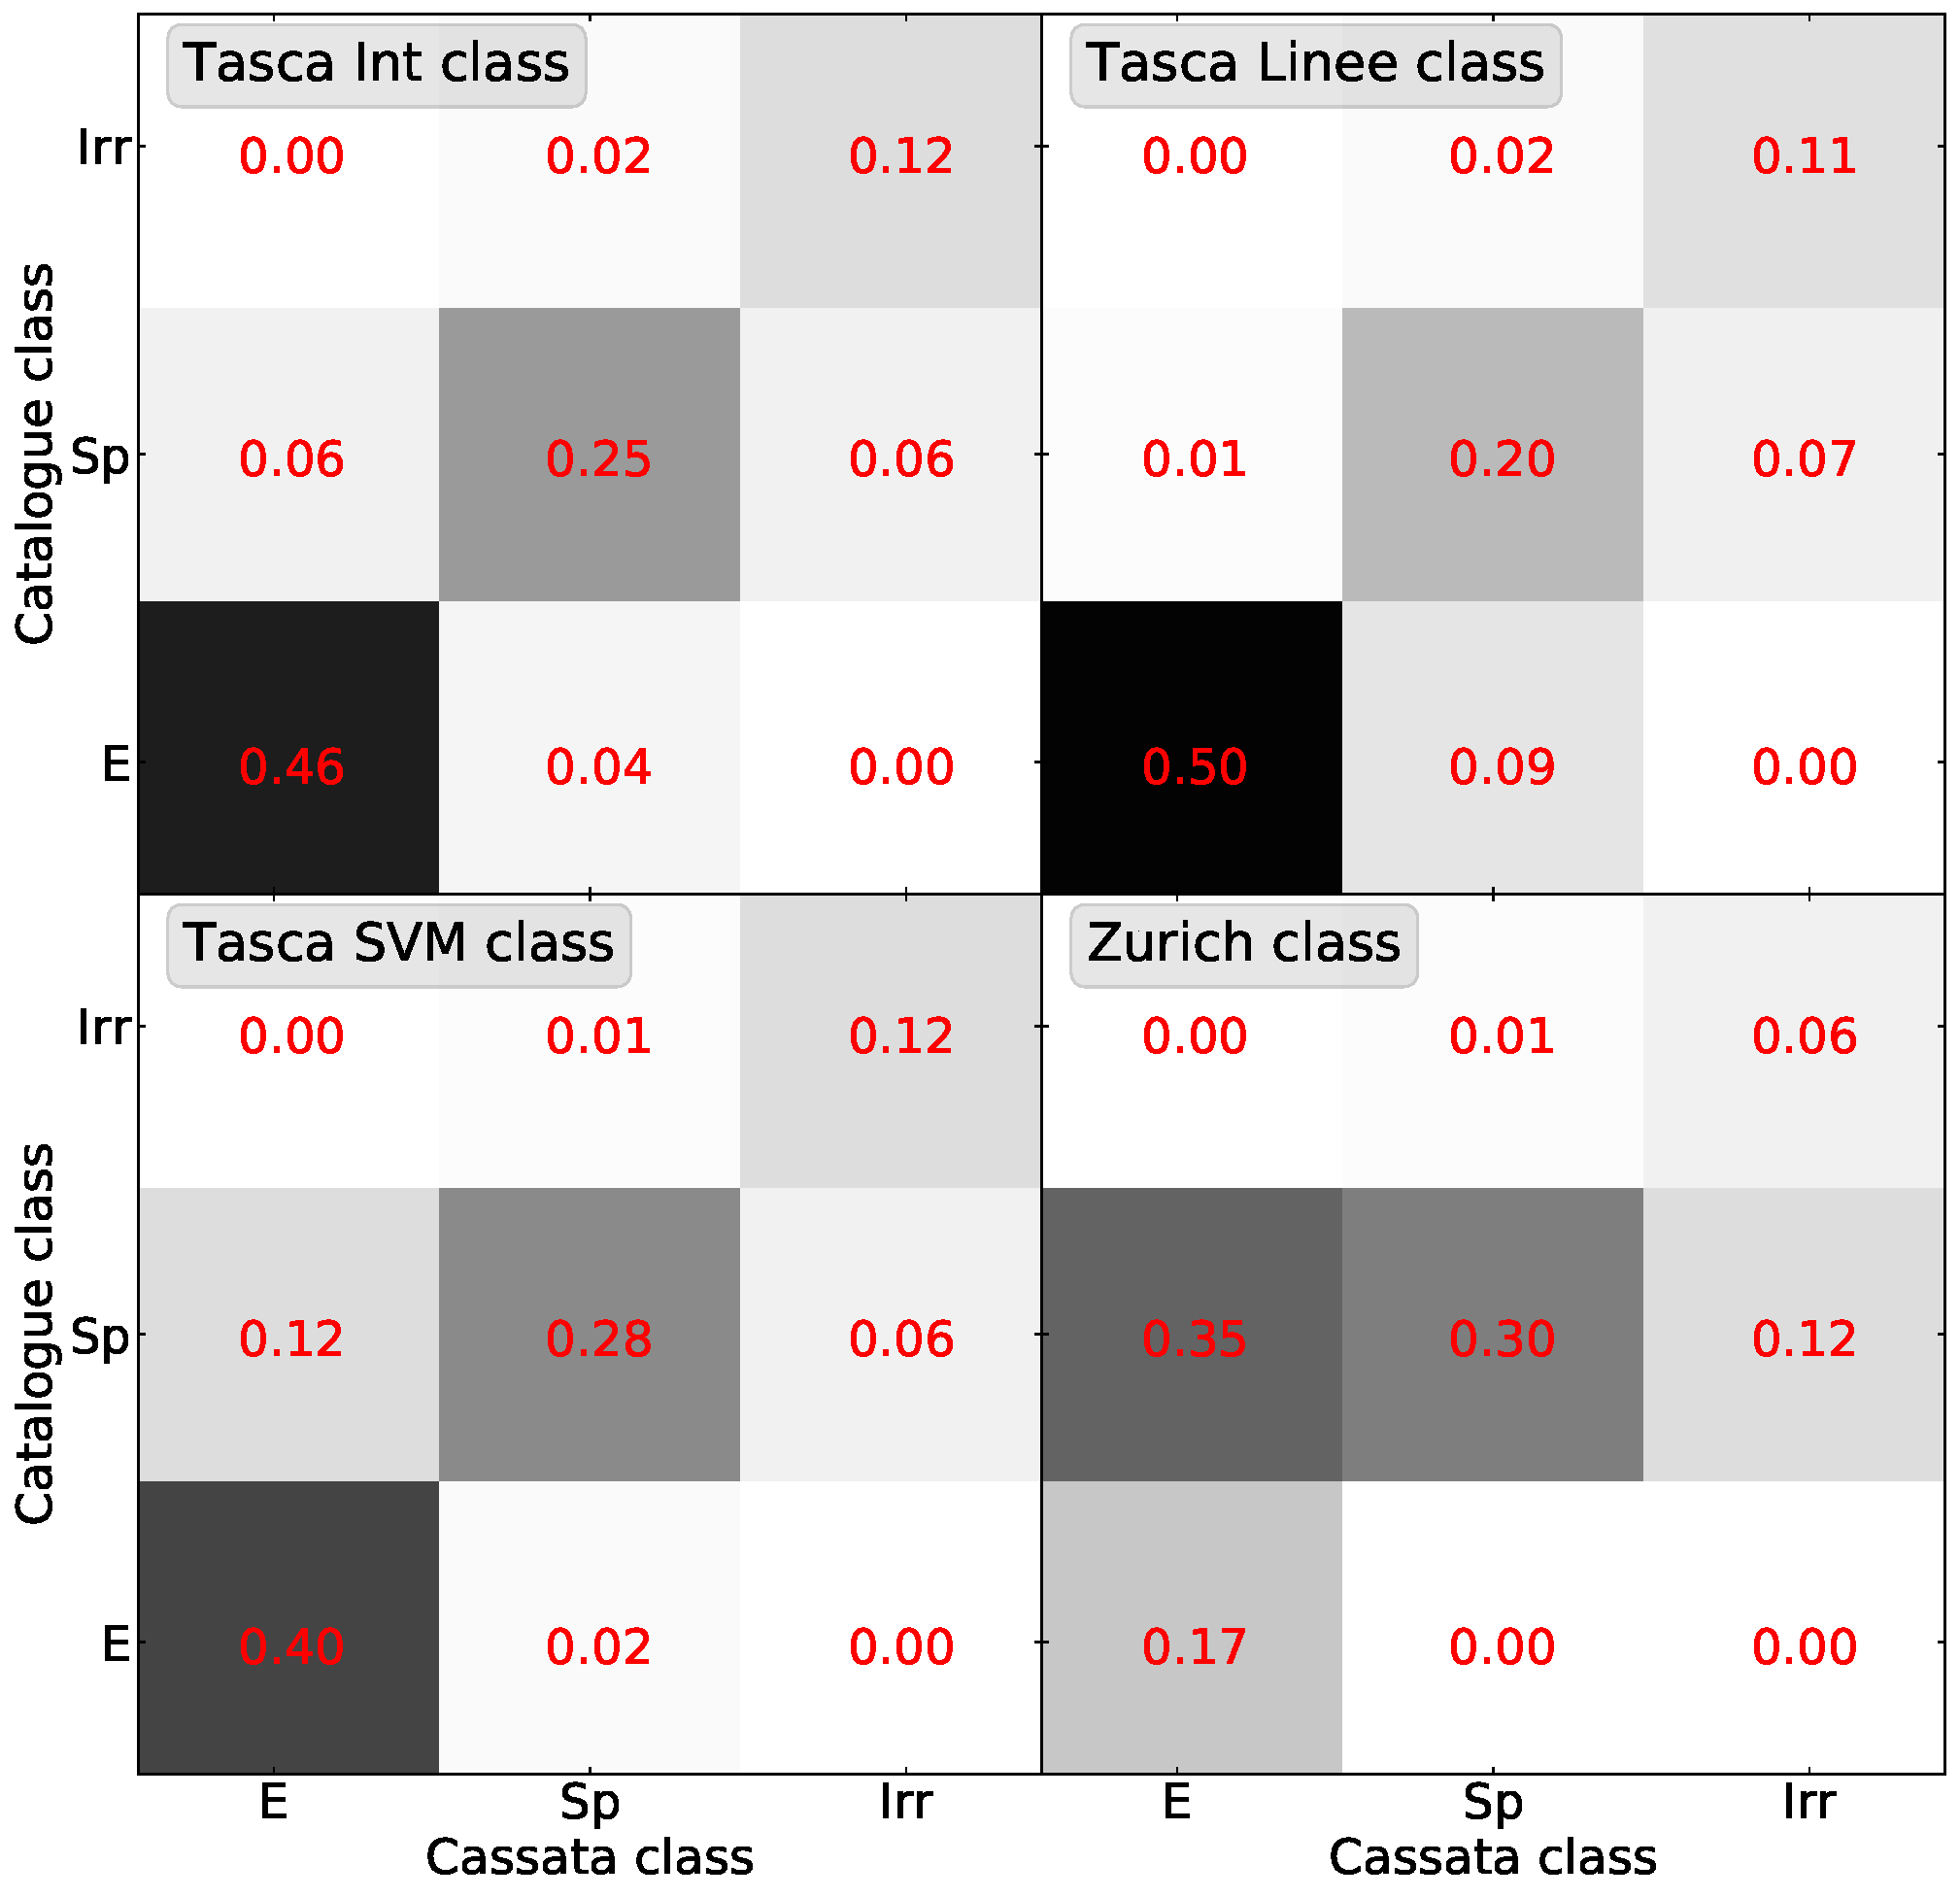
\includegraphics[width=\linewidth]{{../Plots/comparisonClassTypes}.pdf}
	\caption[Morphological types comparison]{Comparison between morphological types given in Tasca and Zurich catalogues against that of Cassata. The three classifications of Tasca are those described in Section\,\ref{subsubsec:classification}. Galaxies are labelled as follows: E for ellipticals, Sp for spirals/disks-like, Irr for irregulars. The percentage of galaxies falling into the given classes is indicated in red and the method compared with Cassata's is shown on the top left corner of each plot. We find good agreement between Tasca and Cassata types but not between Cassata and Zurich.}
	\label{fig:morpho_comp}
\end{figure}

We might expect to have some discrepancies in our data because of the models used between GALFIT and SExtractor/GIM2D. A way to check this effect is to study how these differences scale with the morphological type of the galaxies. For instance, if we use the disk half-light radius of GALFIT to compare with that of SExtractor, we might expect to have some scatter in our relation for the elliptical galaxies as the disk component is not the best one to describe them.\\

To see how these relations scale with morphological types, we can use the classification given in the three morphological catalogues. These classifications are based on methods which can be quite different and which can use morphological parameters in different ways. A more detailed explanation of the parameters used, of how these methods work, of their strength and weaknesses can be found in Appendix \ref{appendix:classification}. We provide below a short introduction to these classifications:

\begin{itemize}
	\item Cassata's catalogue gives a classification based on morphological parameters they derived with SExtractor. To do so, they use a reference of $500$ galaxies with known parameters which they visually classify as either elliptical, disk-like/spiral or irregular. From this set, each time a new galaxy must be classified, its $11$ closest neighbours are inspected and the most frequent class is assigned to the galaxy.
	
	\item Tasca's catalogue gives different classifications based on three methods. The first one is similar to the one used by Cassata. This is also the classification they recommend to use because this is the one they put the more their trust in. The second one uses the technique described in (insert Abraham 1996 here) using the asymmetry and concentration parameters. The last one uses a support vector machine to classify galaxies.
	
	\item Zurich's catalogue gives a single classification called Zurich Estimator of Structural Type (ZEST) which is described in \shortcite{Scarlata2007}. This method is based on a Principal Component Analysis (PCA). They decided to keep the first three Principal Components (PA) which retain most of the information present in the original five parameters (concentration, asymmetry, Gini coefficient, second-order moment of the brightest pixels producing $20\%$ of the total flux and the ellipticity of the galaxy).
\end{itemize}

The morphological types given in Tasca's and Zurich's catalogues are compared against the class given by Cassata in Fig.\,\ref{fig:morpho_comp}. We observe a good agreement between Cassata's and Tasca's types with just a few elliptical galaxies labelled as disk-like and vice versa. Roughly $50\%$ of the galaxies appear to be elliptical. On the contrary, Zurich's classification seems to label more than $70\%$ of the galaxies as disk-like, including a large number of elliptical galaxies .\\

Considering the recommendation of Tasca to use its Int class and since we find a good agreement between Cassata's morphological type and those given by Tasca, we decided to use and to stick to Cassata's class throughout this work whenever we needed to separate galaxies between elliptical/disk-like/irregulars. This choice also ensured us to have the largest sample possible with a coherent classification as Cassata's catalogue is the one with the largest number of HST counterparts of MUSE galaxies in the COSMOS field. Because of the incompatible results between Zurich's and Cassata's/Tasca's types, we decided to put aside these values and not use them, though this shall require further investigation in future work to assess the origin of these discrepancies.

\subsubsection{Half-light radii}
\label{sec:comp_radii}

\begin{figure}[htbp]
	\centering
	\includegraphics[width=\linewidth]{{../Plots/plotsWithColourCoding/relErr_against_galFit1.5LightRadius_colourCoded_matchAllTypes_TwoGalFitRadii}.pdf}
	\caption[Radii comparison between catalogues and GALFIT using bulb and disk]{Relative error on the half-light radius between the catalogues and GALFIT. Points have been colour coded according to their classification given in Cassata's catalogue (Irr for irregular, Sp for spiral/disk, E for ellipticals). Top: GALFIT disk radius is used for all the points. We observe an underestimation of the catalogues radius with respect to that of GALFIT for elliptical galaxies. Bottom: same plot with GALFIT bulb radius used for elliptical galaxies. In this case, we find an overestimation of the radius.}
	\label{fig:comp_radii_with_bulge_or_disk_radius}
\end{figure}

\begin{figure}[htbp]
	\centering
	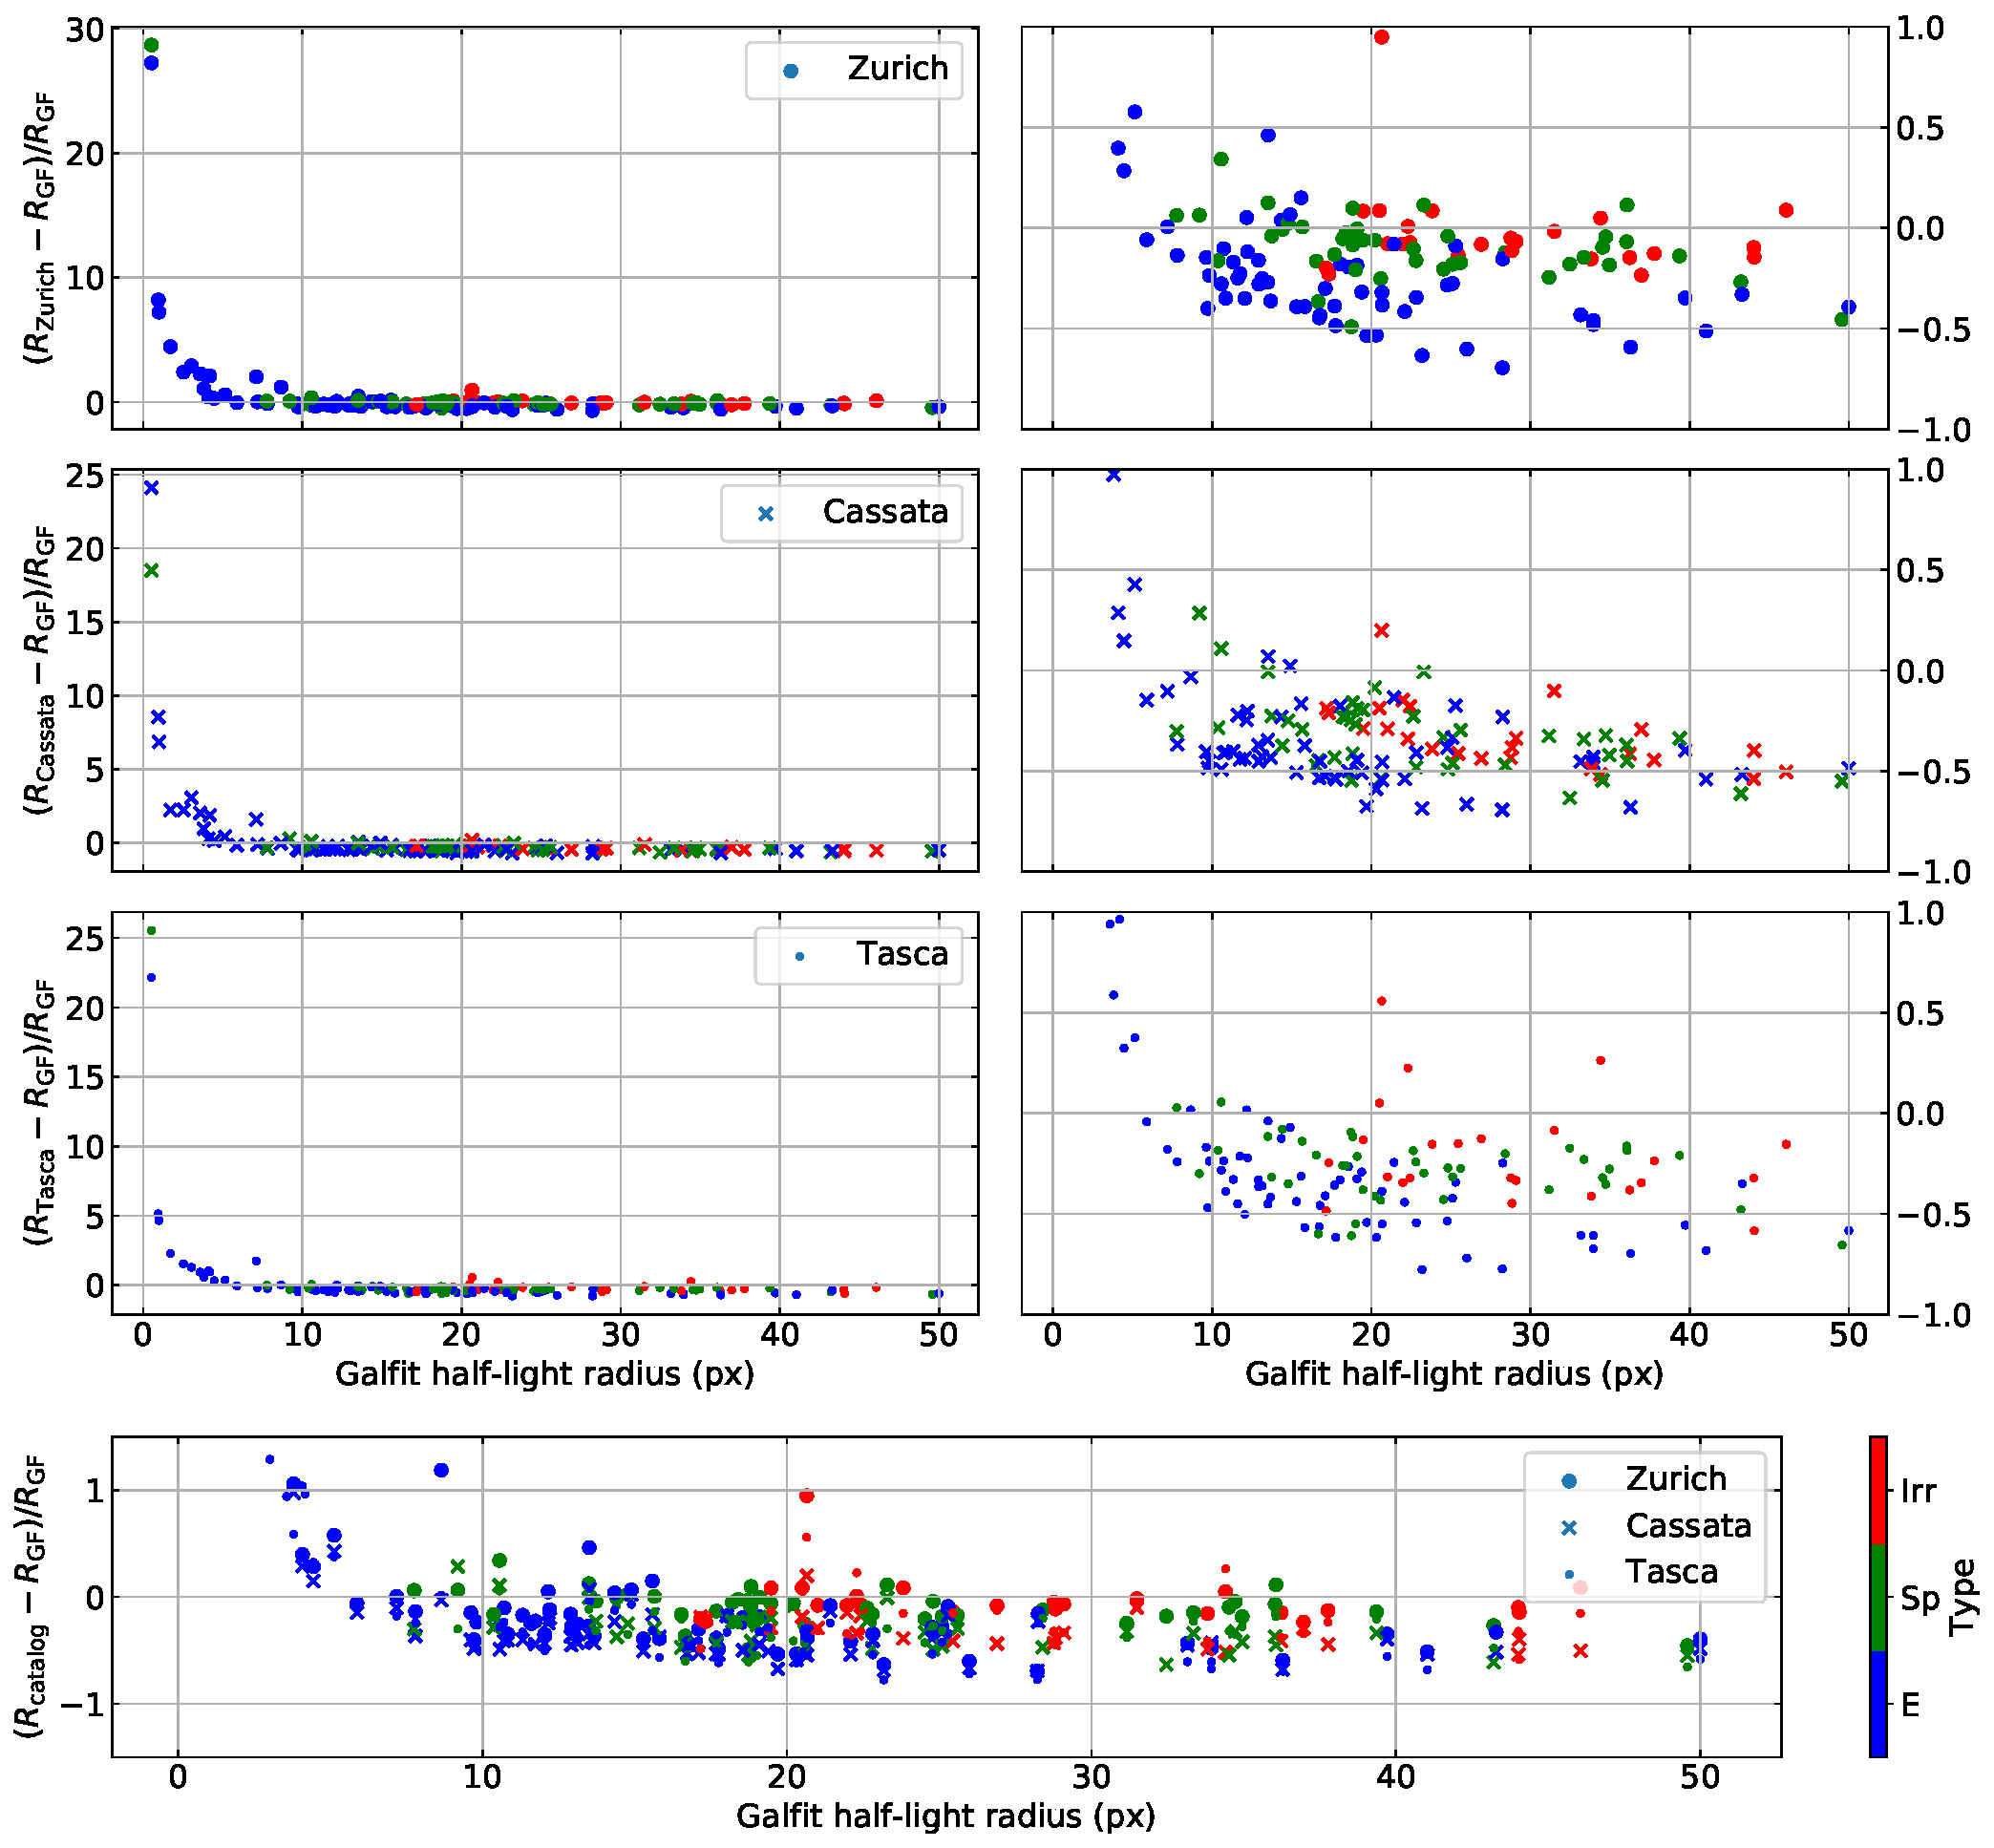
\includegraphics[width=\linewidth]{{../Plots/plotsWithColourCoding/relErr_against_GalFit1.5LightRadius_colourCoded_CassataType}.pdf}
	\caption[Radii comparison per catalogue]{Comparison between half-light radii from the morphological catalogues and the radius of GALFIT disk component. This plot is similar to Fig.\,\ref{fig:comp_radii_with_bulge_or_disk_radius} top plot but each catalogue was separated in its own subplot. Left: full range of relative error. Right: a zoom on the points with $R_{1/2}^{\rm{GF}} \geq \SI{5}{px}$.}
	\label{fig:comp_radii}
\end{figure}

One of the most important parameters we have to check before the selection is the half-light radius of our galaxies. Indeed, if we underestimate it, we might remove from our sample resolved galaxies and therefore reduce our statistics. On the other hand, overestimating it would give us too many unresolved galaxies for which we would spend time performing the cleaning routine without being able to perform their kinematical analysis in the end.
 
Hence, it is mandatory to thoroughly check the values of the half-light radius from the three catalogues against that of GALFIT, and understand the origin of any discrepancies if there happens to be some. \\

We found a quite large disagreement between our GALFIT half-light radius and those given in the morphological catalogues, as well as among them. This is illustrated in Fig.\,\ref{fig:comp_radii} where the half-light radii in the catalogues are compared against that of GALFIT. Galaxies are colour coded according to the classification given in Cassata's catalogue. We checked that using Tasca's classifications as described in Sec.\,\ref{subsubsec:classification} did not change our conclusions. In these plots, we decided to use for the x-axis the half-light radius of the GALFIT disk component for all the galaxies, even though we might expect the ellipticals to be better described by their GALFIT bulge half-light radius.

The catalogues radii seem to be overestimated with respect to that of GALFIT for low $R_{1/2 , \rm{d}}^{\rm{GF}}$. This was expected as catalogues half-light radii are computed using SExtractor. Since it does not take into account the PSF in its fitting routine, we expect the PSF to dominate more for galaxies with small angular sizes. On the contrary, GALFIT does take into account the PSF in its calculations and therefore we expect the half-light radius of GALFIT to be smaller than SExtractor's when reaching low values of $R_{1/2 , \rm{d}}^{\rm{GF}}$. 

When focussing on galaxies with a GALFIT radius larger than the HST-ACS PSF $\rm{FWHM}$ which is around $\sim \SI{0.15}{"}$ ($4 - \SI{5}{px}$), we observe a global underestimation for all the catalogues, up to roughly 50\%. This scatter is mainly due to elliptical galaxies. On the contrary, radii of disk-like galaxies have the least scatter and biais, especially the values given in Zurich's catalogue. This different behaviour between elliptical and disk-like galaxies might be explained, as mentioned above, by the fact we are using the half-light radius of GALFIT disk component to asses the reliability of the elliptical galaxies half-light radii from the catalogues. This is probably not the best choice, and a better may be to use the bulb components, which better describes the light profile of an elliptical galaxy, and its half-light radius to study elliptical galaxies.\\

If we decide to split the galaxies into two categories, ellipticals and disks/irregulars, and if we use for the first category $R_{1/2 , b}^{\rm{GF}}$, and for the second $R_{1/2 , d}^{\rm{GF}}$ we find that elliptical galaxies half-light radii in the catalogues are now overestimated as shown in Fig.\,\ref{fig:comp_radii_with_bulge_or_disk_radius}. This result, and the underestimated values when using the disk radius for the elliptical galaxies, indicates us that elliptical galaxies seem to be neither dominated (in terms of radius) by the disk component, nor by the bulge in the GALFIT model. It is thus necessary to directly compute an overall half-light radius by integrating the galaxies light profile given in Eq.\,\ref{eq:GALFIT_light_profile} \\


CONCLURE SUR QUEL PARAMETRE UTILISER ET QUELLE CORRECTION APPORTER.























\subsection{SNR and size selection}
\label{sec:cut}

\subsubsection{Size selection}
\label{sec:cut_size}

\begin{figure}[t]
	\centering
	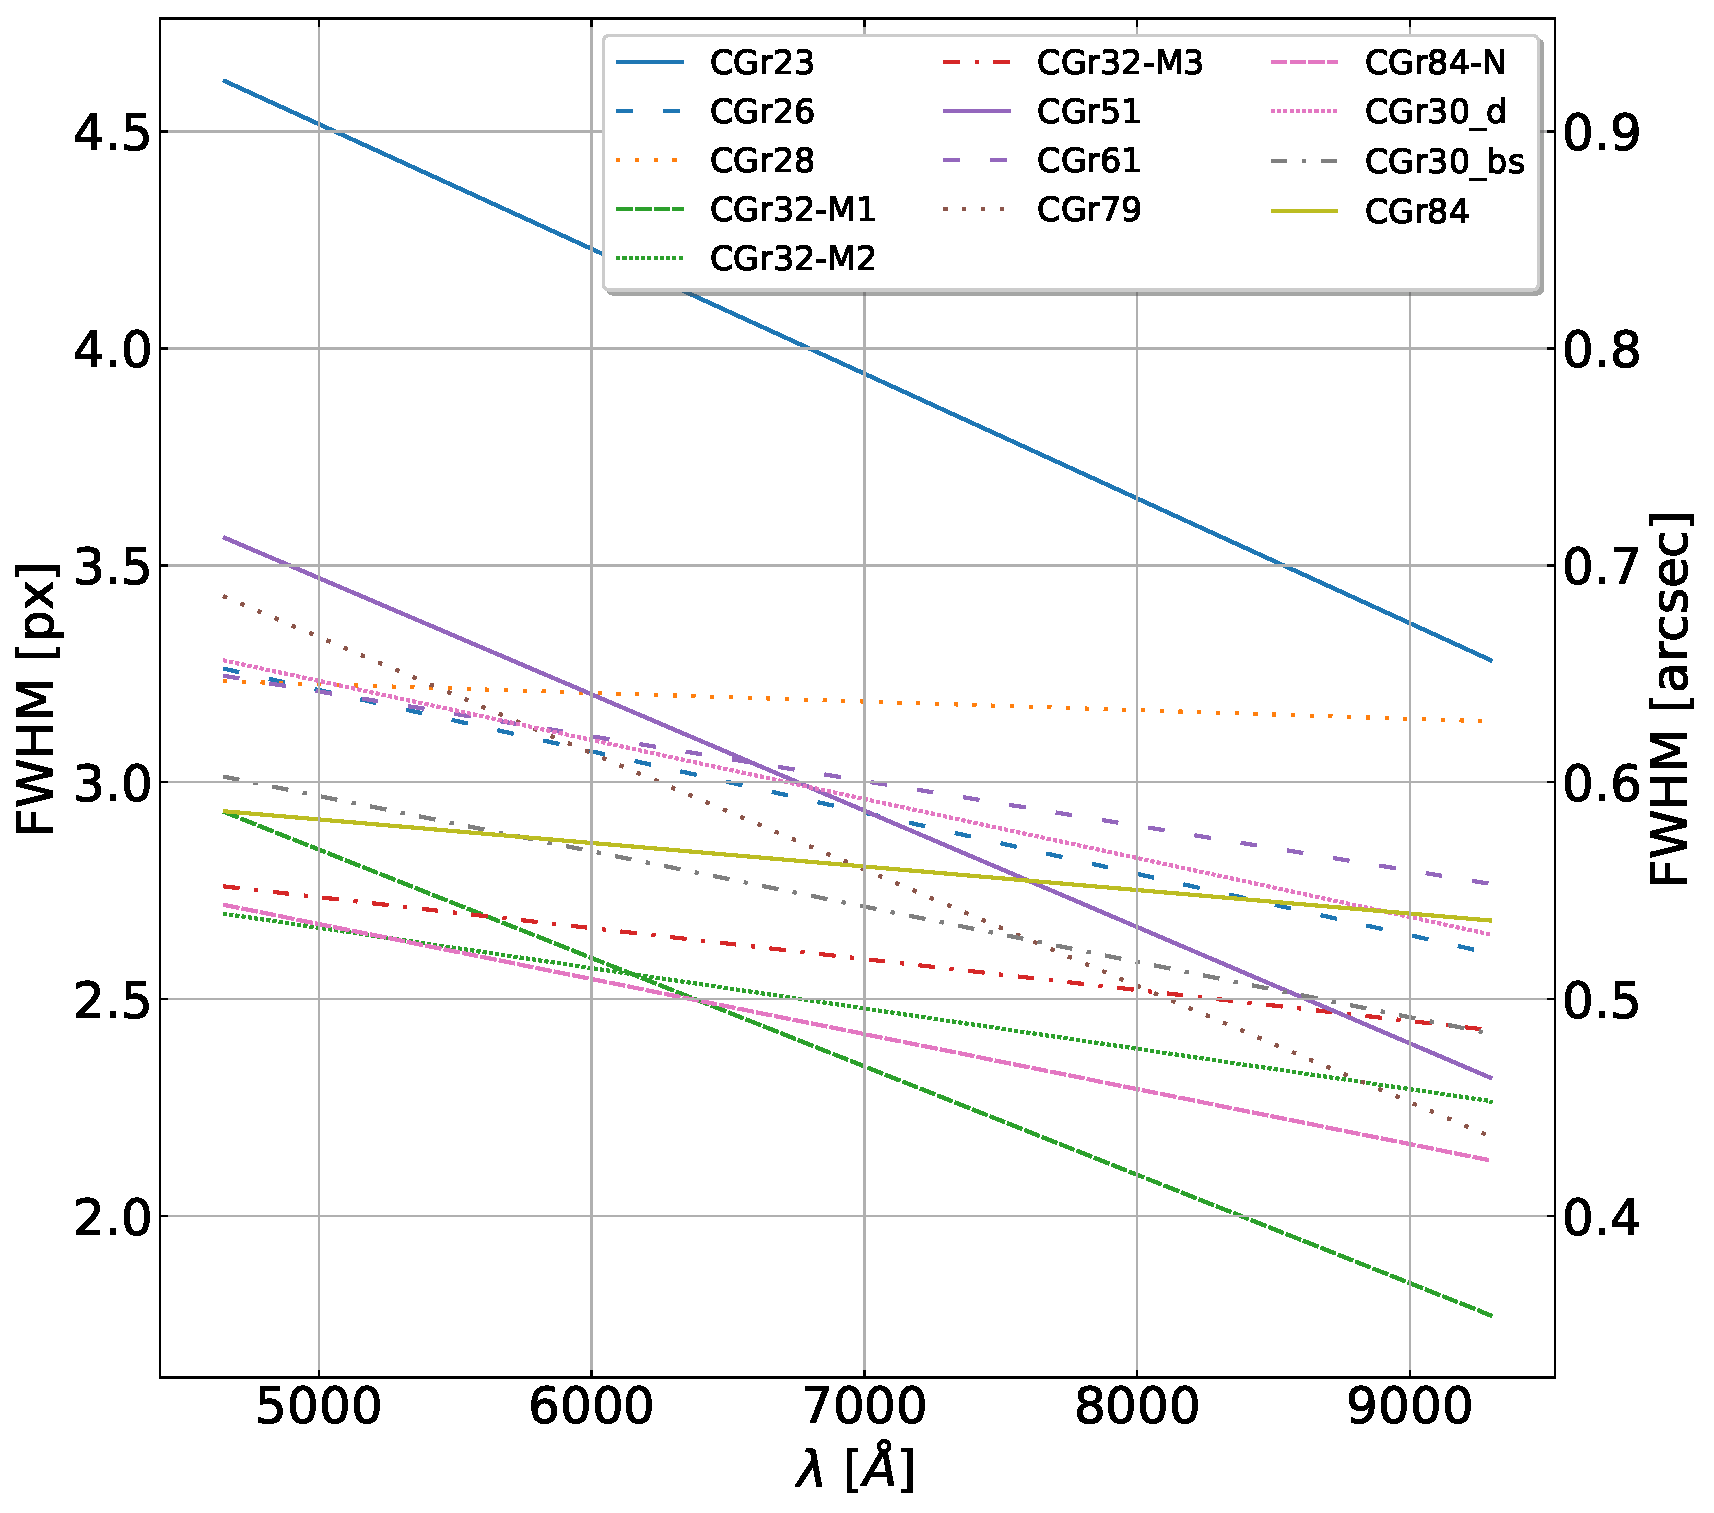
\includegraphics[width=\linewidth]{../Plots/FWHM_variation_with_lambda.pdf}
	\caption[PSF FWHM variation with wavelength.]{PSF FWHM variation with wavelength for the 13 FoVs as measured by Valentina. At least two values of the FWHM were derived from stars in the FoVs by fitting a Moffat distribution to their light profile. We assumed a linear evolution with wavelength. Strong fluctuations appear depending on the observed FoV.}
	\label{fig:FWHM_var_lambda}
\end{figure}

Since we are interested in keeping well resolved field galaxies, we need to apply relevant criteria in order to select the right galaxies. The most obvious parameter we can use to make our selection is the size of the galaxy. We already checked  in Section\,\ref{sec:comp_radii} biases which might arise and their origins, and we corrected them whenever possible. Thus, we only need to define a size criterion to select our sample. \\

Following the earlier work done in \shortciteA{Bacon2015} and \shortciteA{Bacon2017}, the MUSE Point Spread Function (PSF), that is the pattern we obtain when we observe a point-like source with MUSE, is most well described by a \shortciteA{MoffatProfile} profile

\begin{equation}
	I_{\rm{PSF}}(r) = I_0 (1 + (r/\alpha)^2 ) ^{- \beta}
	\label{eq:PSF}
\end{equation}
where $r$ is the radial distance to the centre and $\alpha$, $\beta$ are two seeing dependant parameters. In our case, we are interested in the Full Width at Half Maximum (FWHM) since it is directly related to the seeing conditions and since it gives us information about the minimum spatial extent within which we start to loose information.
The FWHM can be easily derived from the equality $I_{\rm{PSF}} ( \rm{FWHM}/2) = I_0 /2$ using Eq.\,\ref{eq:PSF}, from which we get the following relation

\begin{equation}
	\rm{FWHM} = 2 \alpha \sqrt{2^{1/\beta} - 1 }
	\label{eq:FWHM}
\end{equation}

According to the aforementioned articles the value of $\beta$ is expected to remain roughly constant and, additionally, we would expect from differential image motion theory (insert this paper here when read 10.1086/342683) the FWHM to linearly decrease with wavelength. 

All galaxies are observed via their [OII] doublet at the same rest-frame wavelength. But, given that they are all field galaxies located at a different redshift $z$, we actually observe them at wavelengths covering the entire MUSE spectrum, that is we have the usual relation

\begin{equation}
	\lambda_{\rm{obs}} = \lambda_{\rm{em}} ( 1 + z )
\end{equation}
where $\lambda_{\rm{em}}$, $\lambda_{\rm{obs}}$ are respectively the emitted (rest-frame) and observed wavelengths. Therefore, there is not only one $\rm{FWHM}$ value per field (the $\rm{FWHM}$ will also vary with MUSE fields as seeing conditions change from date to date), but one per galaxy, which we can derive if we know the two parameters (slope and offset) which characterise the linear evolution of the $\rm{FWHM}$ with wavelength. To derive this relation, we need at least two measures of the $\rm{FWHM}$ at two different wavelengths per field. Assuming seeing conditions are similar within a field (no spatial dependence), we can use the same linear relation per MUSE field to compute the $\rm{FWHM}$ for the [OII] wavelength at the redshift of the galaxy. \\

As discussed above, $\beta$ should remain constant, which means the $\rm{FWHM}$ is entirely described by the parameter $\alpha$ through Eq.\,\ref{eq:FWHM}. The measure of $\alpha$ had already been done by V. Abril-Melgarejo on at least two stars per field. For each star, two measures of $\alpha$ were computed by fitting a Moffat profile onto their [OII] and [OIII] images at the redshift of the observed structure (see Table \ref{table:MUSEfieldsProp}).


Though a more rigorous modelling of the wavelength variation of the PSF $\rm{FWHM}$ including both more data points and potentially higher order terms is mandatory for future analysis, we decided to stick to this values in the present work, keeping in mind the large uncertainties which will affect the velocity dispersion maps in the modelling section. A representation of the $\rm{FWHM}$ variation with wavelength for 15 out of 16 observations is shown in Fig.\,\ref{fig:FWHM_var_lambda}. We only have missing values of the $\rm{FWHM}$ for CGr114. Most MUSE fields have $\rm{FWHM}$ values below $\SI{0.7}{"}$ which is not surprising given that it was one of the constraints of the observations. CGr23 is the only FoV to have its $\rm{FWHM}$ above $\SI{0.7}{"}$ for almost every wavelength. Only galaxies further than $z \approx 1.11$. In Table.\,\ref{table:MUSEfieldsProp}, the seeing is the average over the OBs for the [OII] doublet at the redshift of the group which is around $1.17$. Hence the value below $\SI{0.7}{"}$. \\

Considering that the $\rm{FWHM}$ is a measure of how spread a point-like source is, and since we are interested in working with resolved enough galaxies in order to better constrain their kinematics, we would like galaxies to have a characteristic size at least above the $\rm{FWHM}$. Given that for almost all the fields we have an upper limit on the $\rm{FWHM}$ of about $\SI{0.7}{"}$, we decided to use this upper limit as our size selection criterion

\begin{equation}
	R_{1/2} \geq \SI{0.35}{"} \approx \rm{FWHM}/2
\end{equation}

Moreover, according to \shortciteA{Swinbank2017} who compared the half-light radius of the nebular [OII] emission in MUSE images with that of their HST counterpart in ACS \textit{I} or WFC \textit{H}-band, the [OII] half-light radius seems to scale with the HST radius as 

\begin{equation}
	R_{1/2}^{\rm{OII}} = (1.18 \pm 0.03) R_{1/2}^{\rm{HST}}
\end{equation}

Thus, we expect the galaxies in the MUSE images to be larger than their HST counterparts, which means our choice of lower limit for the morphological radius in our sample should eliminate most of the unresolved galaxies. Though, we also risk to eliminate resolved galaxies in our selection.

\subsubsection{SNR selection}
\label{sec:cut_SNR}

The other information we can use to select our sample is the Signal to Noise Ratio ($\rm{SNR}$), which tells us how well our galaxy is detached from the background. The $\rm{SNR}$ is generally derived as the ratio between the source's signal and the background level. The noisier an image, the lower the SNR is.

As explained in later sections, the galaxies must be automatically and then manually cleaned before fitting a kinematical model on the velocity maps in order to remove any pixel dominated by noise which might compromise the fit. One of the criteria used by the routine to decide whether a pixel belongs to the galaxy is a lower limit on the $\rm{SNR}$ of pixel (typically $5$). Thus, if we want to have enough detection in our cleaned maps to perform the kinematical modelling, we must select galaxies with a strong enough SNR.

In our case, \textsc{platefit}, described in \shortciteA{}, was run on the integrated spectrum of the galaxies in order to derive their spectral features. From the parameters returned by CAMEL, we used the [OII] flux and its error to derive the SNR as

\begin{equation}
	\rm{SNR} = \frac{\rm{[OII] \,\, flux}}{\rm{[OII] \,\, flux \,\, error}}
\end{equation}

This is the [OII] $\rm{SNR}$ from the integrated galaxy spectrum computed using pixels within data cubes restricted around the galaxy. Since the typical SNR value used by the routine to clean the maps is around $5$, we decided as a first step to choose an SNR lower limit of $10$, allowing us to keep galaxies with strong enough detection after the automatic cleaning is performed.

\subsection{Characterisation of the sample}

\subsubsection{Selecting galaxies}

\begin{figure}
	\centering
	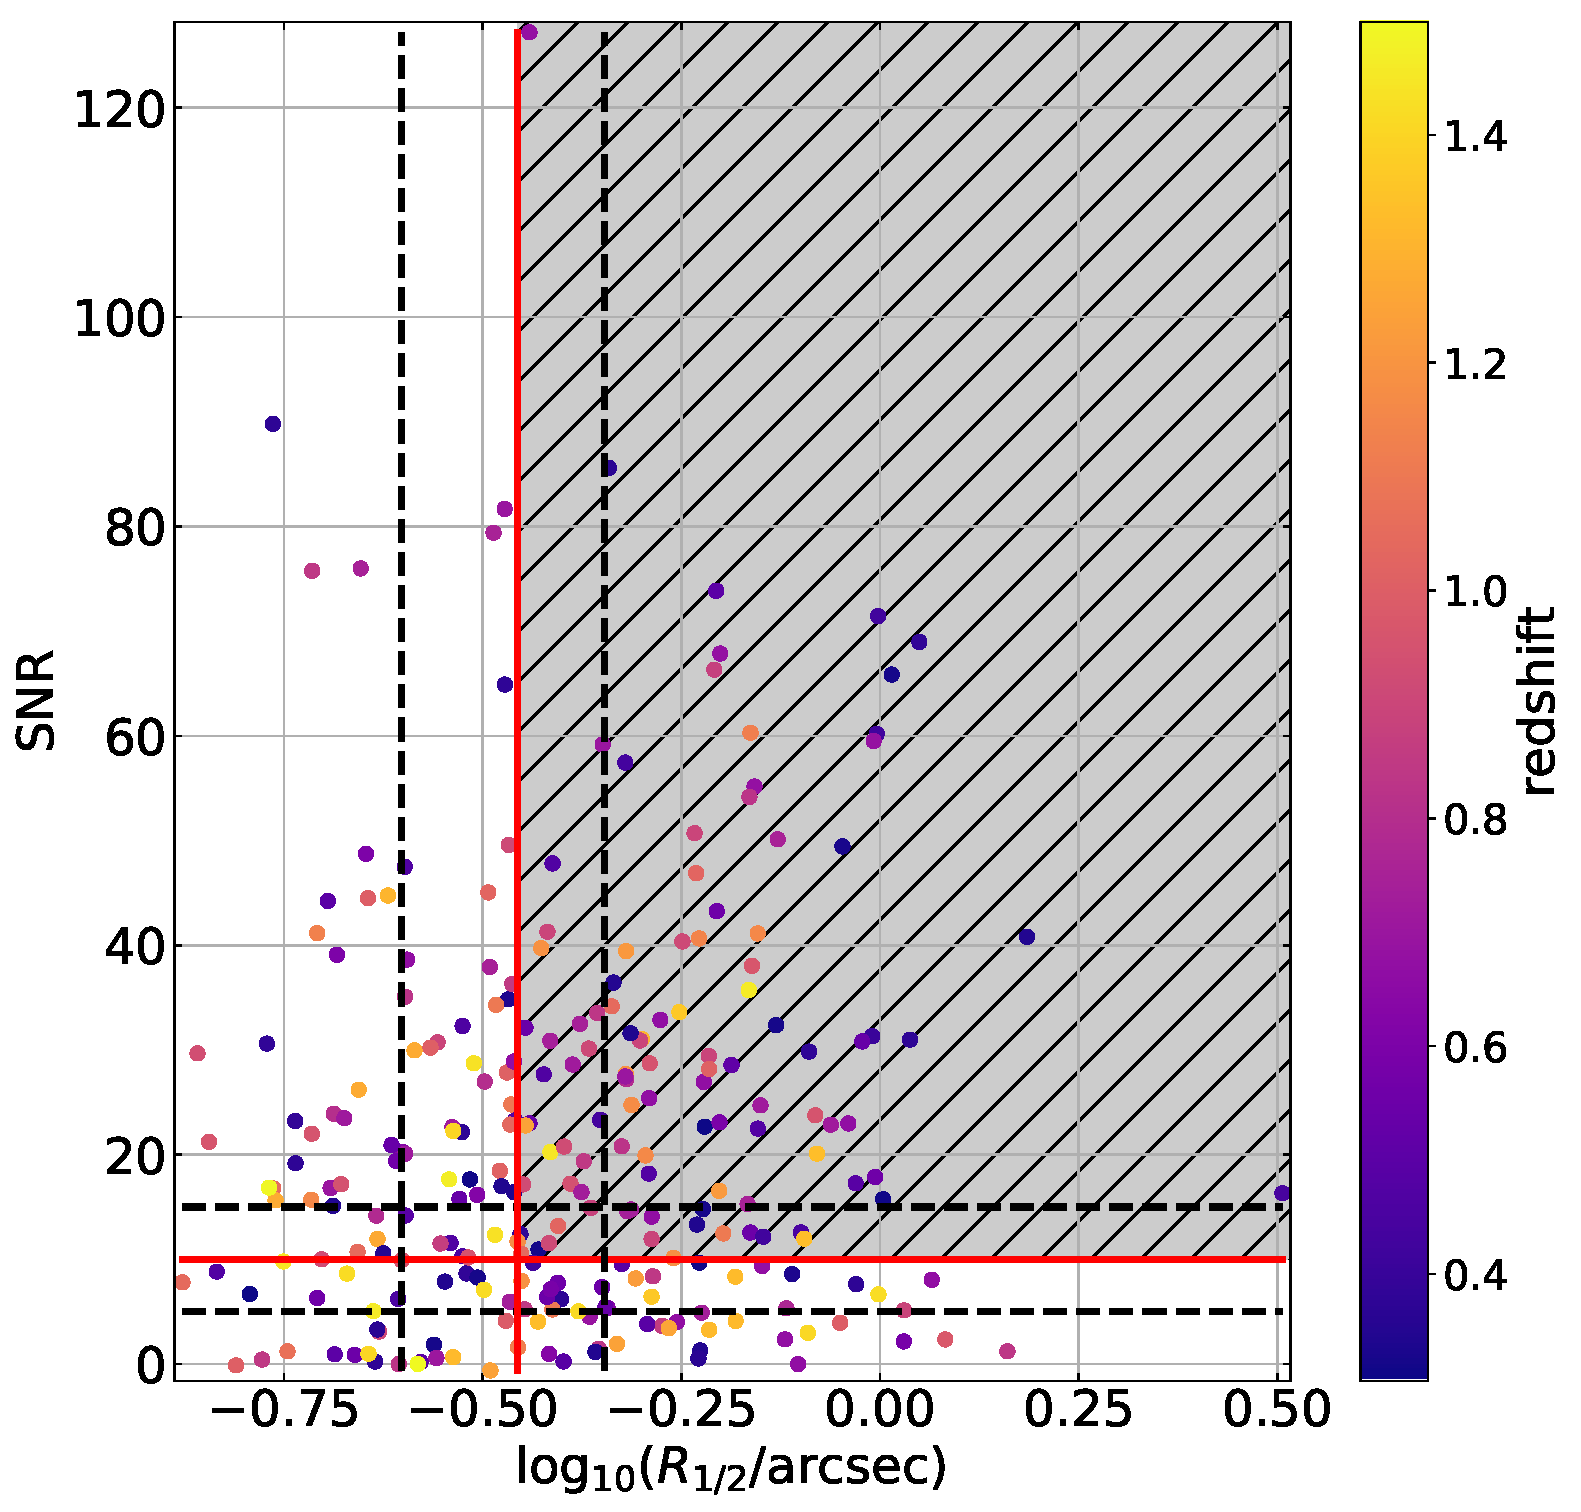
\includegraphics[width=\linewidth]{{../Plots/Selection_plots/SNR_vs_R_halfLight_arcsec}.pdf}
	\caption[Selected sample]{Full sample of $261$ field galaxies with our selection box over-plotted (hatched area). Galaxies with $5 \leq \rm{SNR} \leq 15$ and $0.25" \leq R_{1/2} \leq 0.45"$ (bounds plotted as dashed lines) were visually inspected to check how many resolved galaxies we might have lost. Selection criteria from Sec.\,\ref{sec:cut} are also plotted as solid red lines. No specific trend appear with redshift.}
	\label{fig:sample_selection}
\end{figure}

We decided to visually inspect galaxies around the $\rm{SNR}$ and the size cuts to quantify
\begin{enumerate*}[label={(\alph*)}]
	\item how many resolved galaxies would be lost if we applied the criteria given in Sec.\,\ref{sec:cut_size} and \ref{sec:cut_SNR} (false negative)
	\item how many unresolved galaxies would be selected in our sample (false positive).
\end{enumerate*}
To do so, we defined four boxes: $5 \leq \rm{SNR} \leq 10$, $10 \le \rm{SNR} \leq 15$, $0.25" \leq R_{1/2} \leq 0.35"$ and $0.35" \le R_{1/2} \leq 0.45"$ containing respectively $46$, $20$, $58$ and $49$ galaxies. We then ran the automatic cleaning routine on all the galaxies in these boxes. After visually inspecting their size in the cleaned maps, we classified them as resolved or not. These boxes and the $\rm{SNR}$, half-light radius and redshift of the full sample of field galaxies before selection are shown in Fig.\ref{fig:sample_selection}. \\

Among the $261$ field galaxies, $103$ fall into the limits imposed in Sec.\,\ref{sec:cut}. We find that roughly $26\%$ of the galaxies below the cuts are actually false negatives and that $15\%$ above them are false positives. Since this classification is purely visual, slightly relaxing the constraints on when a galaxy is resolved or not allow these values to vary by roughly $10\%$. Hence, it seems our choice of lower bounds for the $\rm{SNR}$ and the half-light radius is fine, though in future works we might increase our sample by a factor of $\sim 1.5$.

\subsubsection{Redshift distribution}

\begin{wrapfigure}{r}{.5\linewidth}
	\centering
	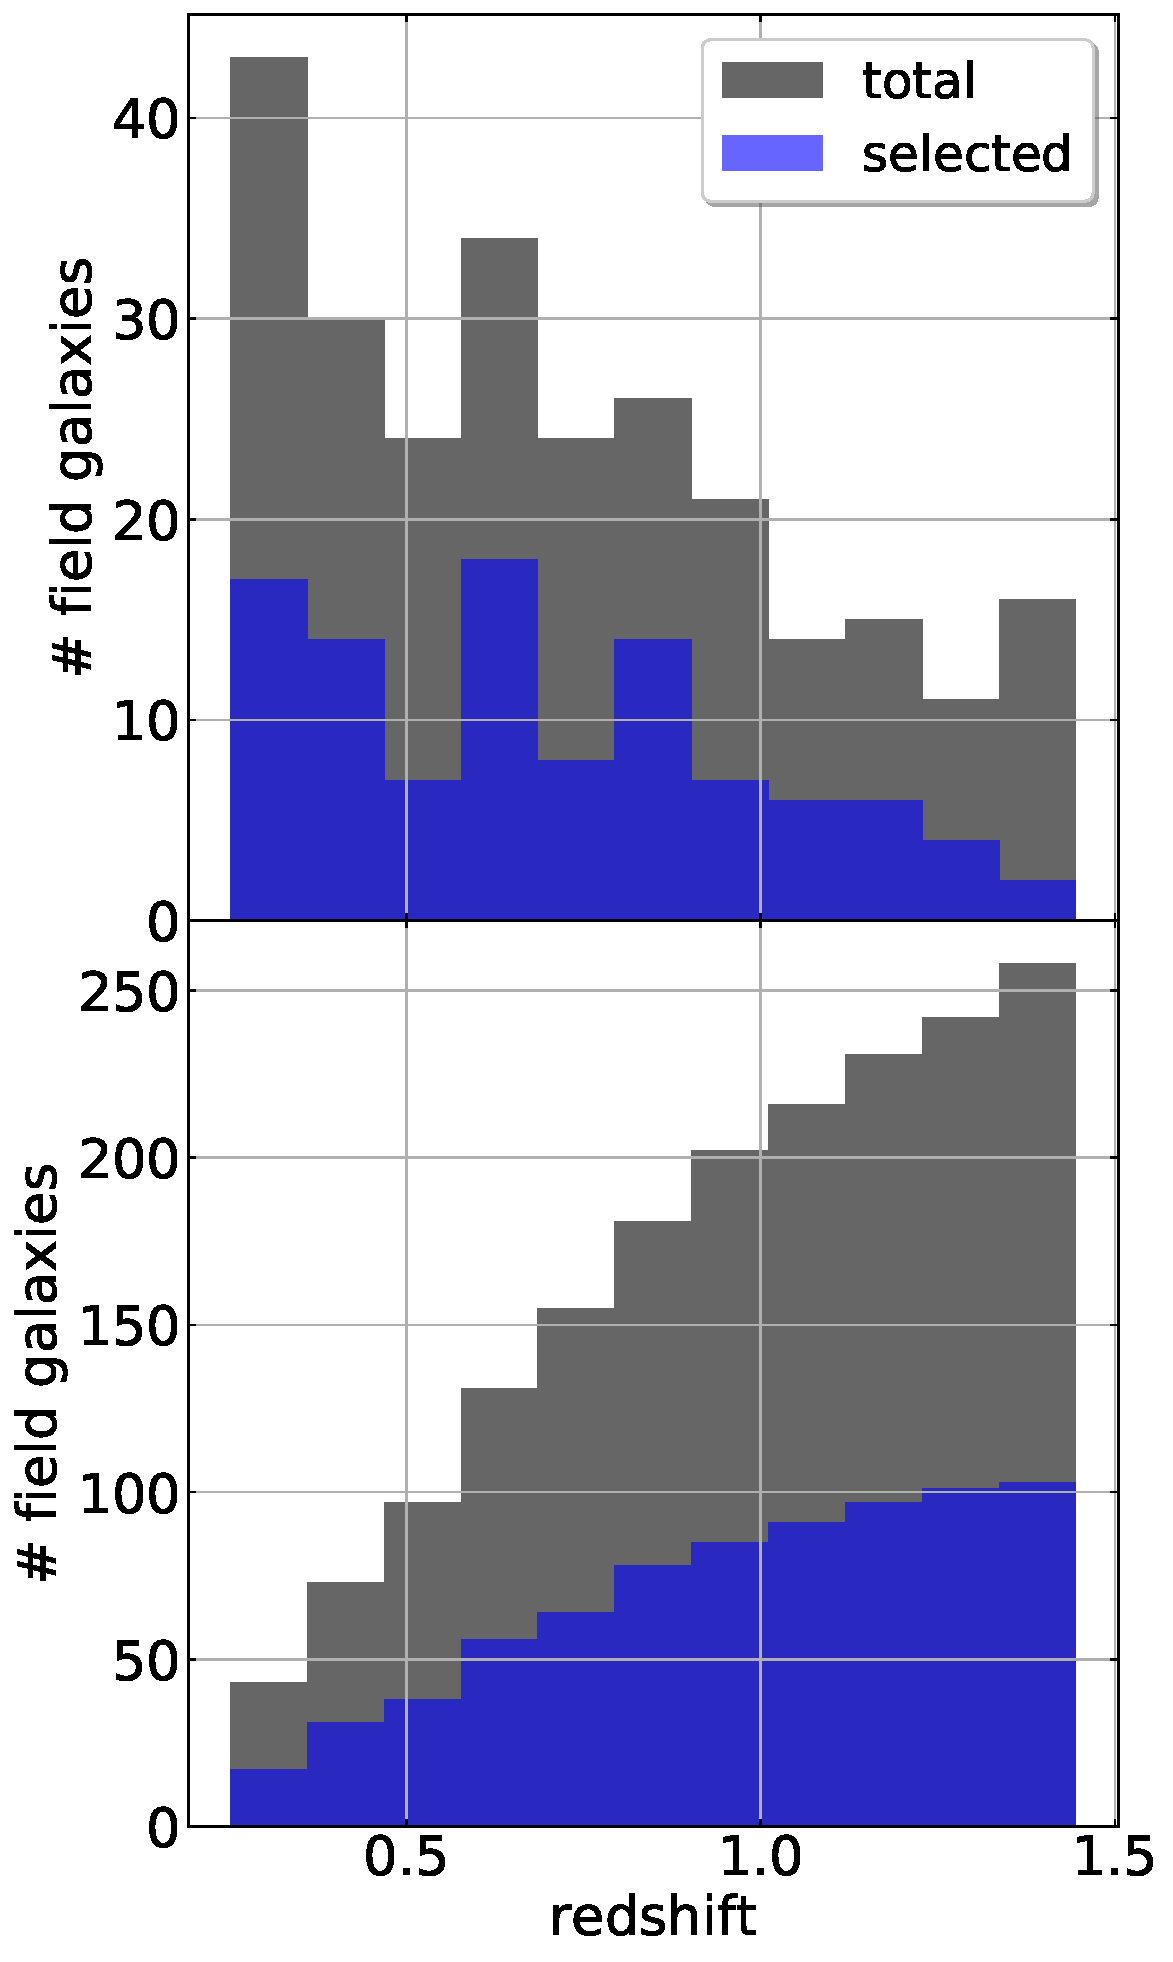
\includegraphics[width=\linewidth]{{../Plots/Selection_plots/cumulative_hist_redshift}.pdf}
	\caption[Redshift distribution]{Redshift distribution of the total sample (grey), selected (green) and unselected (blue) galaxies. Redshift bins of size $0.1$ have been used. Top: density plot as a function of redshift. Bottom: cumulative distribution. We lack most of the galaxies at redshift $1.4$. Other redshift bins do not loose to many galaxies with respect to the unselected ones except maybe at $z \approx 0.5 $.}
	\label{fig:redshift_distribution}
\end{wrapfigure}

The choice of the [OII] $\lambda\lambda 3729, \SI{3729}{\angstrom}$ doublet for the kinematical analysis was due in part to the large range of redshift it covered given the MUSE observed wavelengths. We therefore had in our catalogue galaxies spanning a redshift range from $0.3$ to about $1.4$. As show in Fig.\,\ref{fig:redshift_distribution}, after our selection we loose the majority of the most distant galaxies as well as a significant fraction of galaxies with $z$ around $0.3$, $0.5$ and $0.75$. Globally, we are selecting less galaxies per redshift bin than we are putting aside. The average and median redshifts are $0.749$ and $0.719$ for the selected galaxies, $0.809$ and $0.750$ for the unselected ones. Thus, our sample remains consistent in terms of redshift even after performing the $\rm{SNR}$ and size selections.

\subsubsection{Mass-SFR relation}

\begin{figure}[hbtp]
	\centering
	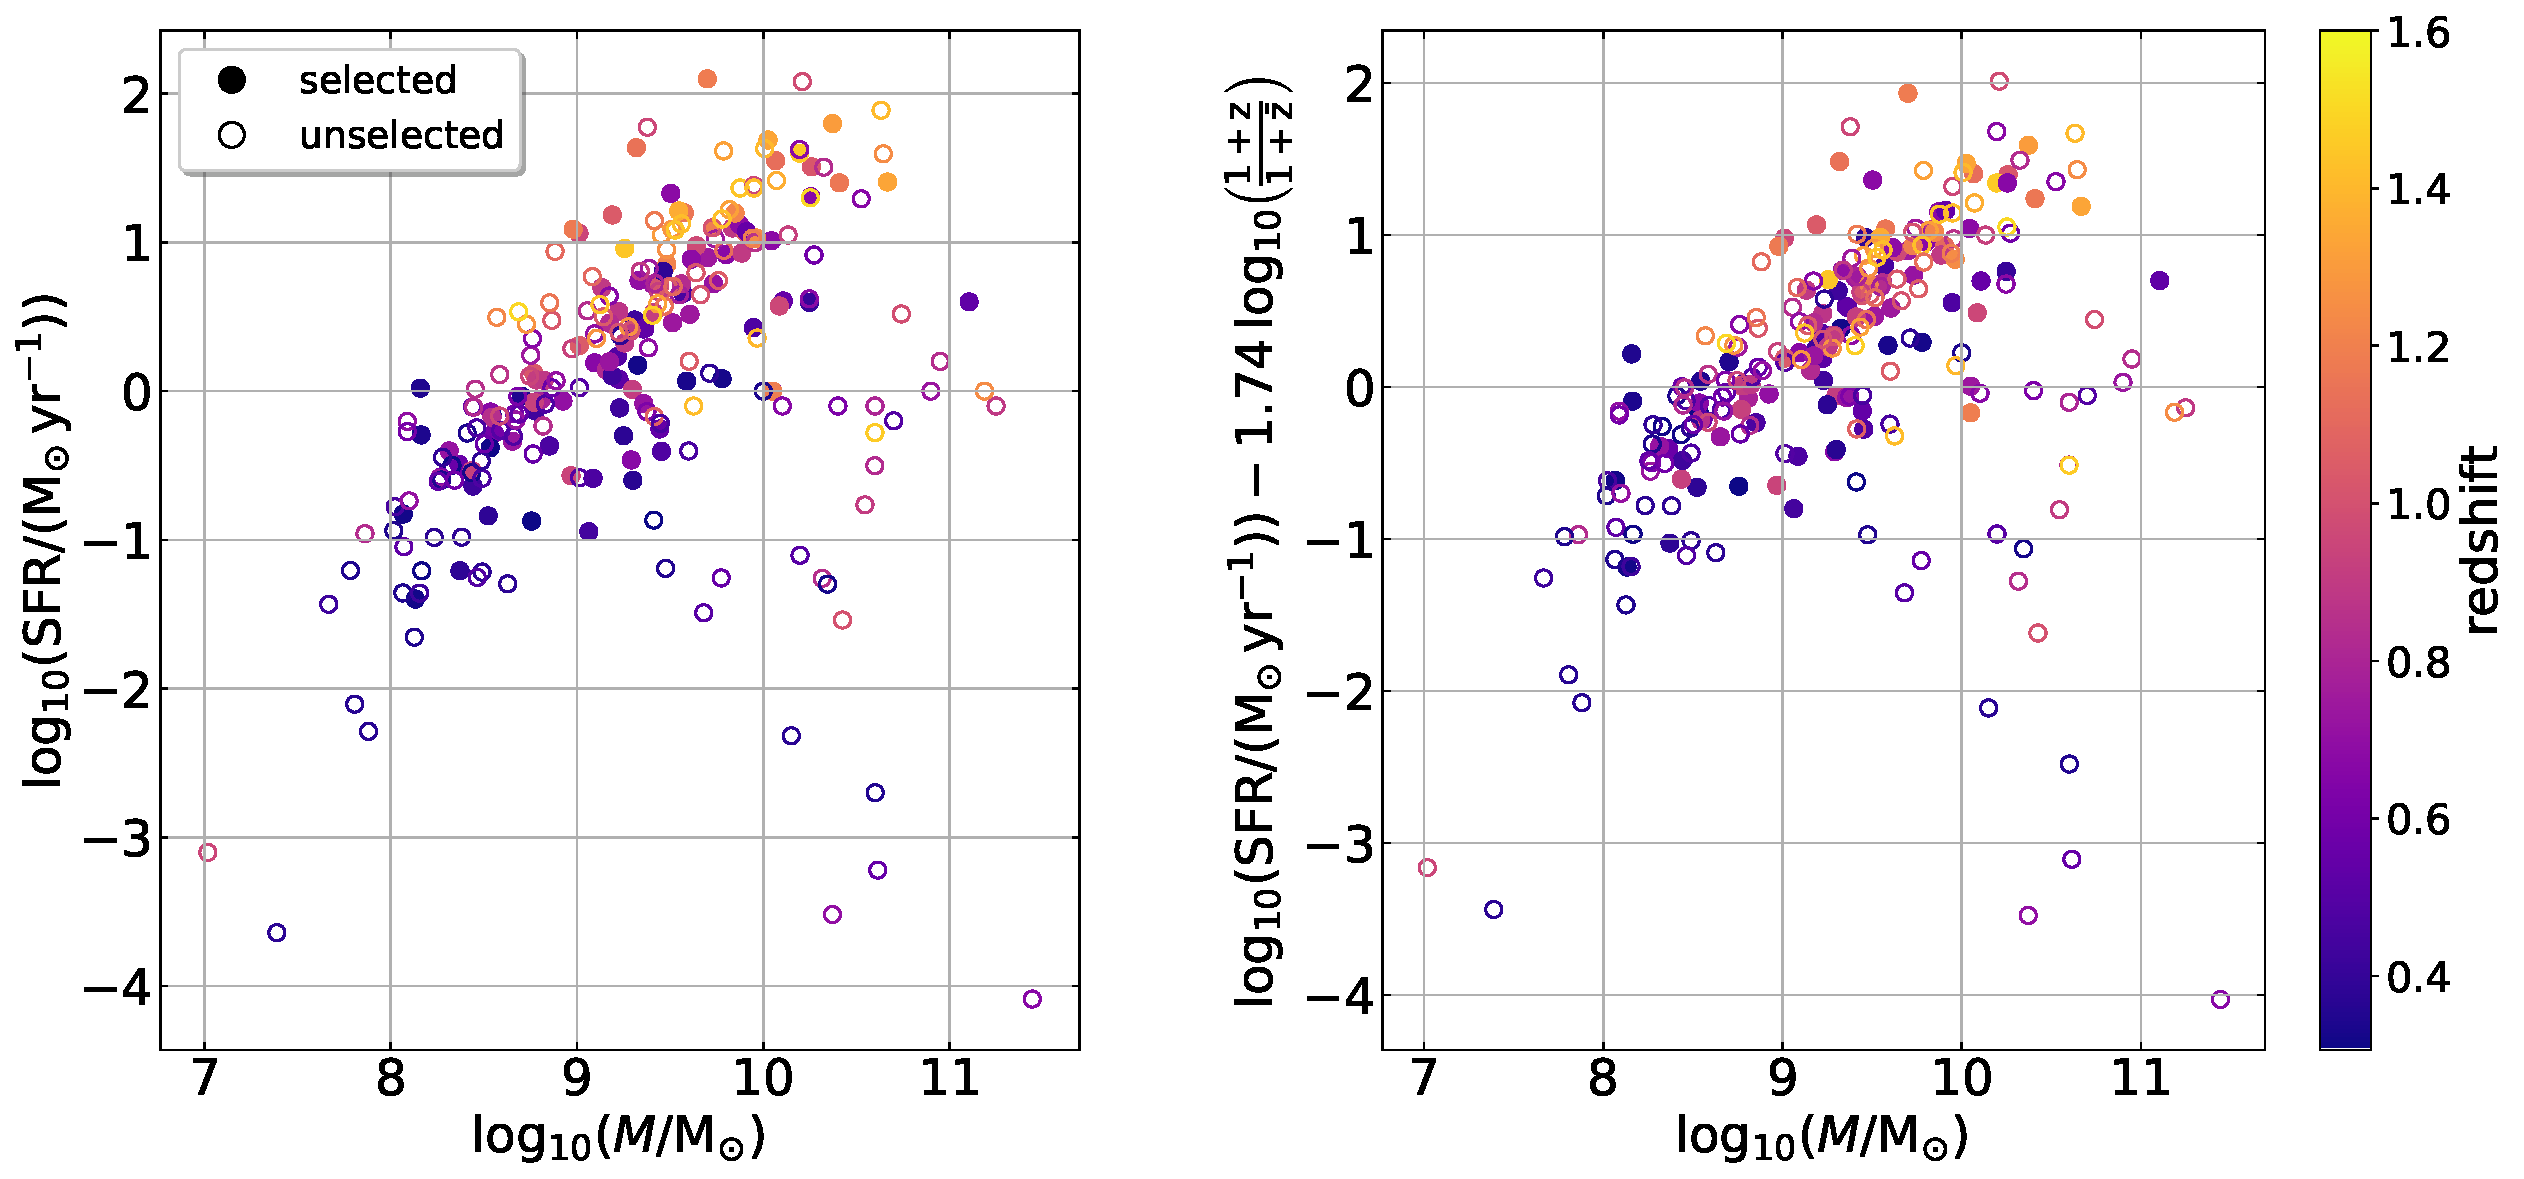
\includegraphics[width=\linewidth]{{../Plots/Selection_plots/SFR_vs_mass_withoutFAST}.pdf}
	\caption[SFR-mass relation]{SFR-mass relation for selected (filled circles) and unselected (open circles) galaxies. Left: SFR extracted from the morphological catalogues. Right: the redshift corrected SFR as given in Eq.\,\ref{eq:SFR_corrected_redshift}. We obtain the usual main sequence of galaxies as a linear relation between SFR and mass (in log-log space), as well as quenched galaxies on the lower right part of the plane which are removed when performing the selection.}
	\label{fig:sfr_vs_mass}
\end{figure}



 
